\documentclass[12pt]{ctexart} % 使用 ctexart 文档类支持中文

\usepackage{fancyhdr} % 奇特的 header
\usepackage{xcolor} % 更多颜色

\usepackage[utf8]{inputenc} % 支持 UTF8 字符,在 UTF8 engine 中无需此行
\usepackage{xeCJK} % 支持中文排版,已经包含在 ctexart 中
\usepackage{fontspec} % 字体设置
\usepackage{geometry} % 页面布局
\usepackage{titlesec} % 自定义标题样式
\usepackage{setspace} % 设置行距
\usepackage{microtype} % 更多的微调
\usepackage{tabularx} % 表格支持
\usepackage{booktabs} 
\usepackage{float} % Add the float package,支持图片位置固定

\usepackage[colorlinks,linkcolor=black,urlcolor=black]{hyperref} % 超链接支持

\usepackage{tocloft} % 自定义目录样式

\usepackage{graphicx} % 图片设置
\graphicspath{ {./images/} }

% 设置页面布局
\geometry{a4paper, margin=1in}

% 设置行距为 1.25 倍
\setstretch{1.25}

% 设置中文字体
\setCJKmainfont{SimSun}[BoldFont={Microsoft YaHei Bold}] % 设置正文为宋体

\setCJKsansfont{Microsoft YaHei}[BoldFont={Microsoft YaHei Bold}] % 标题等无衬线字体为黑体

% 设置英文字体
\setmainfont{Times New Roman}



% 配置页眉和页脚
\pagestyle{fancy}
\fancyhf{}

\renewcommand{\headrulewidth}{0pt}

\setlength{\headheight}{25.60938pt} % Set the headheight to the required value
\addtolength{\topmargin}{-13.60938pt} % Adjust the topmargin to compensate

% 定义颜色
\definecolor{myred}{RGB}{244, 67, 54} % 蓝色

% 左侧页眉设置, 页码在页眉外侧
\fancyhead[L]{%
  \colorbox{myred}{%
    \parbox[t]{1cm}{%
      \textcolor{white}{\thepage}%
    }%
  }%
  \hspace{0.5cm}
  总体报告v2.0
}

% \fancyhead[L]{\leftmark} % 左页显示章节名

% 页眉横线设置
\renewcommand{\headrulewidth}{0.5pt}
\renewcommand{\headrule}{%
  \hbox to\headwidth{%
    \color{black}\leaders\hrule height \headrulewidth\hfill%
  }%
}

% 页脚页数设置
\renewcommand{\footrulewidth}{0pt}
\fancyfoot[C]{\thepage}

% 设置目录样式
\renewcommand{\cftsecfont}{\bfseries} % 目录中章节标题加粗

\titleformat{\section}
  {\normalfont\Large\bfseries} % 移除 \centering
  {\thesection}{1em}{}


% 超链接设置
\hypersetup{
  colorlinks=true,
  linkcolor=black,
  filecolor=magenta,      
  urlcolor=magenta,
}

\begin{document}

\begin{titlepage}
  \centering % 居中对齐
  % \vspace*{1cm} % 从顶部添加一些垂直间距
  
\includegraphics[width=0.6\textwidth]{zjutitle.jpg} % 插入图片
  
  \vspace{2cm} % 添加垂直间距
  
  {\fontsize{36}{48}\selectfont\CJKfontspec{Microsoft YaHei} 总体报告v2.0} % 标题
  
  \vspace{2cm} % 添加垂直间距
  
  
\includegraphics[width=0.4\textwidth]{zjulogo.jpg} % 插入图片
  
  \vspace{2cm}
  
  {\Huge\CJKfontspec{Microsoft YaHei} 项目主题: \underline{H5游戏分享平台}} % 项目主题 with underline
  
  \vspace{1cm}

  {\Large\CJKfontspec{Microsoft YaHei} 第 1 小组: \underline{XXX}} % 作者
  
  \vspace{1cm} % 添加垂直间距
  
  {\Large\CJKfontspec{Microsoft YaHei} \today} % 日期

\end{titlepage}

\newpage
\tableofcontents % 自动生成目录
\newpage


\section{需求分析}

\subsection{项目背景}
该项目开发的软件为一个HTML5 游戏分享平台。随着互联网技术的发展,HTML5
技术凭借其跨平台兼容性、无需插件加载、即点即玩的特性,已成为游戏开发与传播的
重要载体。传统游戏平台更多面向客户端或主机游戏,而轻量化、低门槛的HTML5 游
戏往往分散于各类网站或社交媒体中,缺乏统一的展示、体验与互动空间。在此背景下,
构建一个专注于HTML5 游戏的在线分享平台,既是技术发展的必然趋势,也是满足用
户需求的关键举措。

相较于传统游戏分发模式,HTML5 游戏分享平台让玩家随时随地通过浏览器畅玩
游戏,同时为开发者提供低成本、高效率的作品展示渠道。对玩家而言,平台可汇聚海
量创意游戏,通过标签分类、用户评分与社区推荐快速发现优质内容;对开发者而言,
平台既能成为技术交流的窗口,又能通过用户反馈优化作品,甚至实现商业化潜力;此
外,随着教育领域对编程与游戏化教学需求的增长,该平台还可作为教学案例库,助力
游戏爱好者学习游戏开发技术。

在互联网时代,游戏行业的技术风向与用户偏好瞬息万变,而游戏社区就是游戏发
展壮大的土壤,是游戏不断进步的根基。HTML5 游戏分享平台能够构建动态交互社区
生态:玩家可实时分享攻略、录制精彩片段;开发者能发布技术日志、参与话题讨论;
平台也会进行数据分析,为游戏优化提供依据。最终能形成“创作-体验-反馈”的良性
循环。

\subsection{用户类及其特征}
实际产品进行了交付后的产品使用方拥有三种角色,我们将其定义为三个用户类,
分别为管理员、普通用户、游客。如表\ref{tab:usertable}所示。

\begin{table}[htbp]
    \centering
    
    \begin{tabular}{|p{2cm}|p{10cm}|}
        \hline
        用户 & 描述\\
        \hline
        管理员 & 管理员拥有H5游戏分享平台的最高权限,负责系统的日常运行,可以以对所有游戏的情况进行查看,以及负责对新上传游戏的审核,同时管理所有普通用户的账户信息。此外管理员可以对网站网页的部分静态内容进行自由编辑。 \\
        \hline
        普通用户 & 管理员创建普通用户账号,所有普通用户都拥有上传游戏以及游玩游戏的权限,游戏开发者可以按照格式上传自己开发的游戏,并进行版本管理,撰写游戏介绍,发布游戏公告,开放下载等权限;游戏玩家既可以在网页端直接游玩游戏,也可以下载到本地。 \\
        \hline
        游客 & 游客只拥有在网页端游玩游戏的权限。\\
        \hline
    \end{tabular}
    \caption{用户类及其特征}
    \label{tab:usertable}
\end{table}

\subsection{产品功能}
产品使用者可分为上述的三种用户,依照各个用户所拥有的权限,H5 游戏分享平台的功能如表\ref{tab:productfunction}所示。

  \begin{table}[htbp]
      \centering
      \begin{tabular}{|p{3cm}|p{3cm}|}
          \hline
          产品功能 & 设计的用户类别\\
          \hline
          游戏审核与数据收集 & 管理员\\
          \hline
          游戏发布与更新 & 普通用户\\
          \hline
          游戏游玩 & 普通用户,游客\\
          \hline
          发表评论 & 普通用户\\
          \hline
      \end{tabular}
      \caption{产品功能}
      \label{tab:productfunction}
  \end{table}

\section{整体设计}
\subsection{体系结构设计}
在软件工程中,体系结构风格是用于定义软件系统高层次结构和组织模式的抽象框
架。它是一种通用的、可复用的解决方案,用于在特定上下文中组织软件系统的结构与
交互方式,描述了系统组件的类型、组件间的交互方式、约束条件以及适用的场景,为
设计决策提供指导原则。

一个体系结构风格通常包括:组件类型(系统由哪些功能模块组成),连接件类型
(模块之间如何通信),拓扑结构(组件和连接件的组织方式),语义约束(对交互方式、
数据流动、控制流的限制)。

体系结构风格是设计系统的“蓝图”,选择时需要权衡利弊,结合具体场景灵活应
用。为了找到适合我们软件的体系结构风格,我们参考了以下常见的体系结构风格:
\begin{itemize}
  \item 以数据为中心的体系结构
  \item 数据流体系结构
  \item 调用和返回体系结构
  \item 面向对象的体系结构
  \item 层次体系结构
  \item 客户端-服务器架构
  \item 浏览器-服务器架构
  \item 微服务架构
  \item 事件驱动架构
\end{itemize}
本次设计的“HTML5游戏分享平台”是一款基于浏览器-服务器(B/S)模式的网页应用,同时以多媒体文件系统为中心,因而兼具B/S体系架构和典型的数据中心架构特点。

平台的客户端完全运行在用户的浏览器中,用 HTML5/TypeScript 渲染游戏列表、详情页及分享交互界面;服务器端则提供静态资源托管和多媒体流等服务。
\begin{enumerate}
  \item 客户端(Browser):负责页面渲染、用户交互捕获(评论、点赞等等),并与服务器通信。
  \item 服务器(Server):接收并处理前端请求,执行业务逻辑、访问数据库和文件系统,最终返回JSON数据或媒体流给客户端。
\end{enumerate}

所有游戏包、截图、演示视频等大容量多媒体文件统一存储在专用的文件存储系统或对象存储服务中,平台各组件通过同一仓库访问和更新这些资源:
\begin{enumerate}
  \item 存储层:包括文件服务器、CDN 缓存,以及元数据数据库(存储文件路径、大小、格式、关联游戏 ID 等)。
  \item 数据访问层:封装对元数据表的操作,并提供获取下载链接、上传凭证等接口。
\end{enumerate}

这种“中心化”的文件管理模式,符合数据中心架构风格,能够简化多媒体资源的共享与一致性维护。

同时,用户“上传游戏”、“点击游玩”、“发表评论”等操作,均通过触发事件,由事件处理器异步处理,这也体现出事件驱动架构的一部分特征。

综上所述,“HTML5游戏分享平台”以B/S 架构为基础,通过数据中心架构集中管理多媒体资源;
同时结合了事件驱动等多种体系架构风格,形成了具备高内聚、易扩展、可维护性强的现代化平台架构。

\subsection{体系结构环境图和原型}
体系结构环境图展示了系统的边界以及系统与其环境中的其他组件之间的关系。
这有助于确保所有相关组件得到适当的关注,以便实现一个完整和可靠的系统。
通过展示系统与其所在环境和业务需求之间的关系,体系结构环境图可以帮助设计人员确保所设计的系统与实际需求保持一致。

在明白外部的因素之后,我们对模型内部进行设计,还需要挖掘模块中核心的抽象类或者模式,此即原型。
原型设计有助于更早地发现和解决设计中的问题和不足之处,从而降低项目风险和成本。
通过与用户进行原型测试,设计人员可以获取宝贵的反馈,以便对系统进行改进和优化。
原型设计有助于确保最终系统满足用户需求,提高系统的质量和性能。
通过迭代的原型设计过程,设计人员可以更快地调整和完善系统功能,从而缩短开发周期。

本节展示了H5游戏分享平台系统的体系结构环境图和原型,体现了系统与其环境中的各种组件之间的关系和互动。
\subsubsection{视图层}
视图层基于Next.js框架搭建,负责呈现用户界面并处理用户交互。其体系结构环境图如下;

\begin{figure}[htbp]
  \centering 
  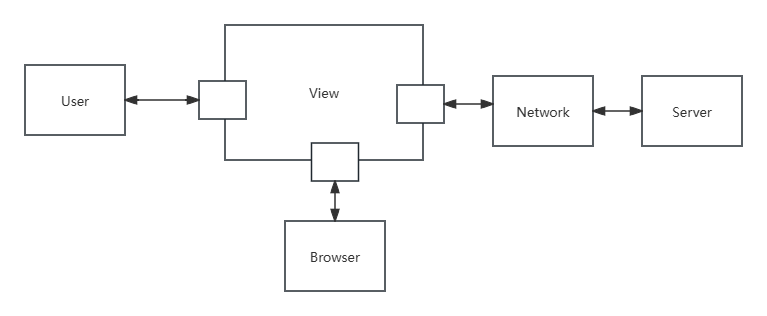
\includegraphics[width=0.8\textwidth]{view.png}
  \caption{视图层}
\end{figure}

视图层采用组件化设计,主要功能包括:

1、游戏列表展示

2、游戏详情页渲染

3、游戏上传表单处理

4、用户个人信息展示

5、与服务器端的数据交互

视图层通过API与服务器端通信,接收数据并在浏览器中渲染。对于游戏内容,视图层会嵌入相应元素。
\subsubsection{控制层}
控制层是系统的核心业务逻辑处理单元,采用FastAPI框架实现。其体系结构环境图如下:

\begin{figure}[htbp]
  \centering 
  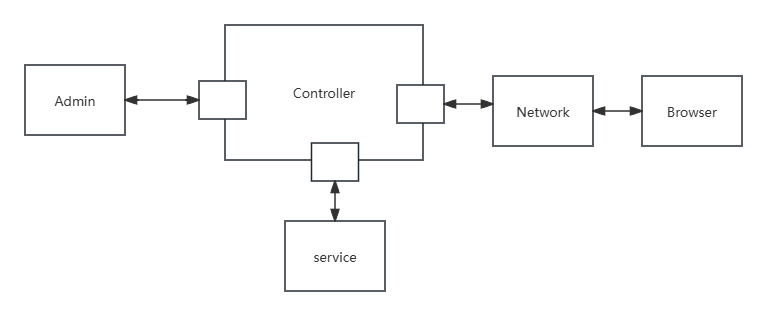
\includegraphics[width=0.8\textwidth]{control.png}
  \caption{控制层}
\end{figure}

1、控制层的主要职责包括:

2、接收并验证HTTP请求

3、处理身份认证和授权

4、调用适当的服务层组件

5、格式化响应数据

6、处理错误和异常
\subsubsection{服务层}
服务层包含系统的核心业务逻辑模块,其体系结构环境图如下:

\begin{figure}[htbp]
  \centering 
  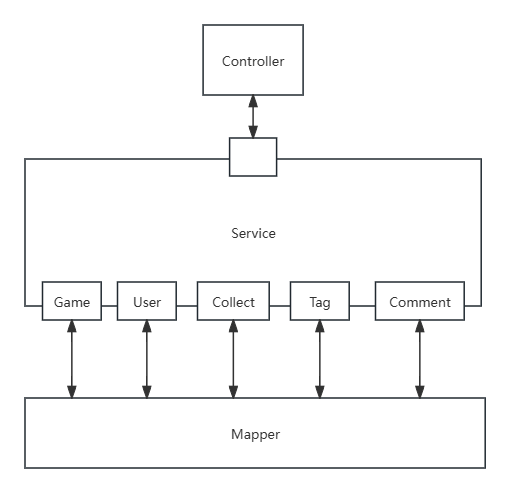
\includegraphics[width=0.8\textwidth]{service.png}
  \caption{服务层}
\end{figure}

服务层通过数据访问层与数据库和文件存储系统交互,确保业务逻辑与数据持久化分离。

\subparagraph{游戏管理模块}

该模块主要负责对游戏信息的管理。包括游戏的上传,查看,游玩,下载,更新功能。普通用户可以
进行游戏的上传,查看,游玩,下载。游戏创作者以及管理员可以实现对游戏的更该。
该模块主要具有以下几个功能:

处理游戏上传、更新和删除

管理游戏元数据

处理游戏文件存储

生成游戏预览和截图

\begin{figure}[htbp]
  \centering 
  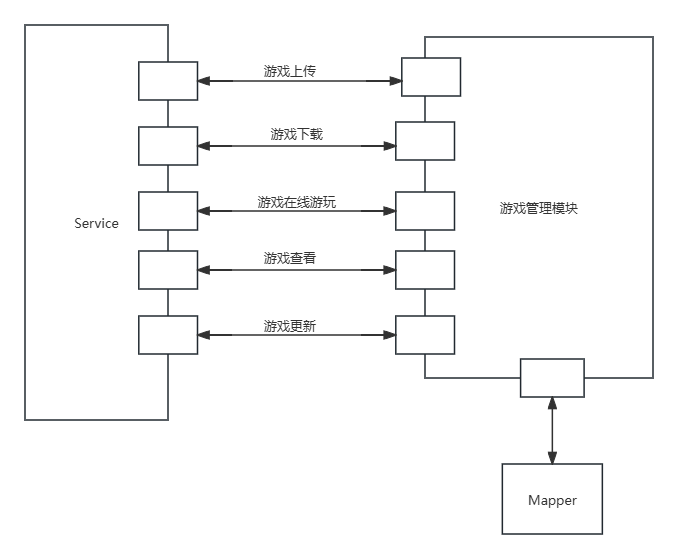
\includegraphics[width=0.8\textwidth]{game.png}
  \caption{游戏管理模块}
\end{figure}

\subparagraph{标签管理模块}

该模块主要负责对标签信息的管理。包括游戏与标签的匹配,标签本身的管理功能。
管理员可以实现对标签的管理。
该模块主要具有以下几个功能:

管理游戏分类标签

处理标签关联关系

提供标签筛选功能

\begin{figure}[H]
  \centering 
  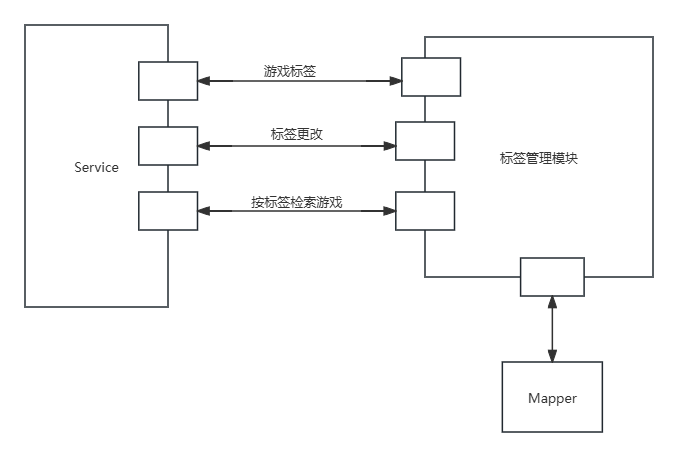
\includegraphics[width=0.8\textwidth]{tag.png}
  \caption{标签管理模块}
\end{figure}

\subparagraph{收藏管理模块}

该模块主要负责对用户收藏信息的管理,以支持用户收藏游戏,管理收藏,查看收藏的功能。
从而增加用户的使用便捷度。
该模块主要具有以下几个功能:

处理用户收藏行为

管理收藏关系

提供收藏列表

\begin{figure}[htbp]
  \centering 
  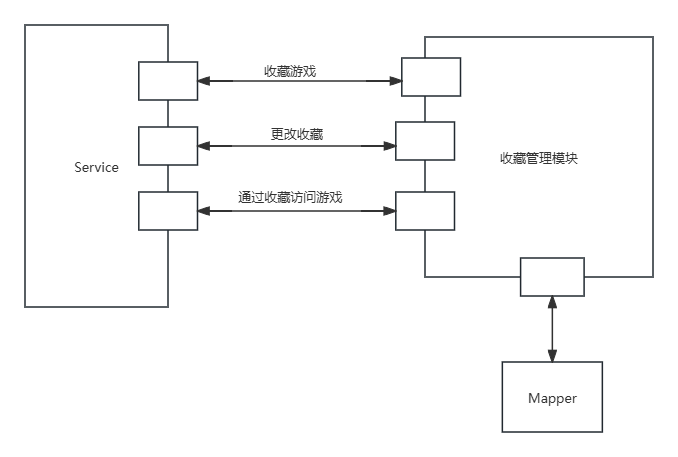
\includegraphics[width=0.8\textwidth]{collect.png}
  \caption{收藏管理模块}
\end{figure}

\subparagraph{用户管理模块}

该模块主要负责对用户信息的管理,实现用户的登录与注册,管理用户自身资料的功能。
该模块主要具有以下几个功能:

处理用户认证

管理用户资料

处理用户行为统计

\begin{figure}[htbp]
  \centering 
  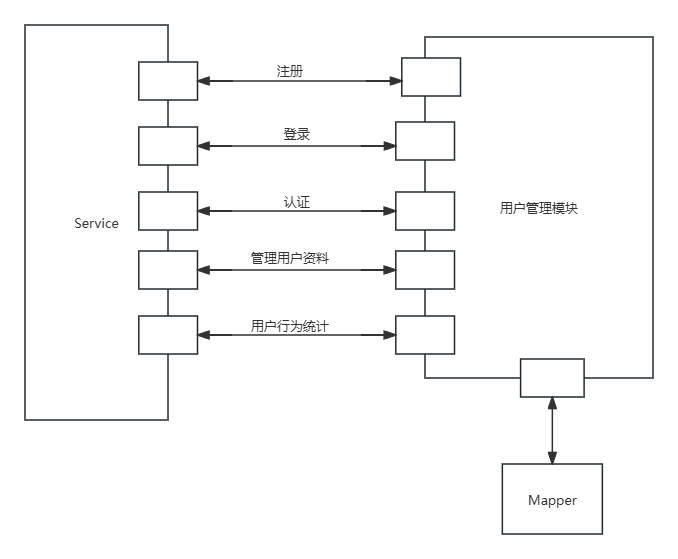
\includegraphics[width=0.8\textwidth]{user.png}
  \caption{用户管理模块}
\end{figure}

\subsubsection{模型层}
映射层和模型层在项目中起着至关重要的作用,它们分别负责数据访问和数据模型的定义。
通过这种分层架构,可以实现业务逻辑与数据库操作的解耦,提高代码的可维护性和可扩展性。

\paragraph{映射层}

Mapper 层主要负责数据库访问操作。它包含了与数据库进行交互的相关接口和方法,
如插入、删除、更新和查询等。 Mapper 层的主要目的是将业务逻辑层与数据库操作解耦,
使得业务逻辑层更关注业务逻辑的实现,而不需要关心数据库操作的具体实现细节。映射层体系结构环境图如下

\begin{figure}[htbp]
  \centering 
  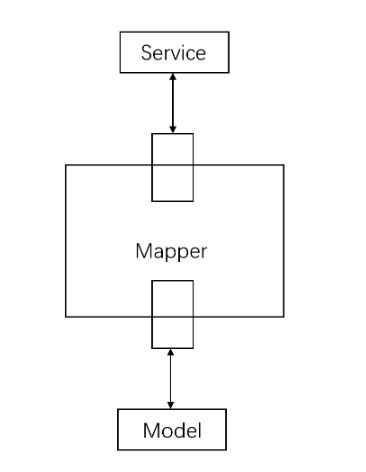
\includegraphics[width=0.4\textwidth]{map.png}
  \caption{映射层}
\end{figure}

\paragraph{模型层}
模型层定义系统的数据结构和持久化机制,确保数据的一致性和完整性,同时提供高效的数据访问接口给服务层使用。
通过清晰的模型定义,系统可以更好地组织和管理核心业务数据。

\begin{figure}[htbp]
  \centering 
  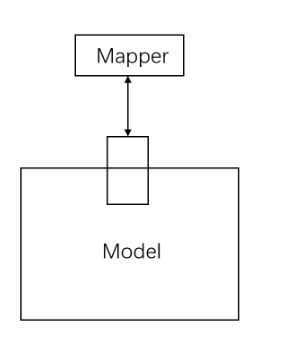
\includegraphics[width=0.4\textwidth]{model.png}
  \caption{模型层}
\end{figure}

\subsection{数据处理流程}
以下按不同业务列出处理流程:
\begin{enumerate}
  \item 上传游戏:从请求体中获取到对应信息,加入文件库,并且向数据访问层提交数据库修改请求。
  \item 获取游戏列表:从数据访问层获取到对应的游戏列表,并且返回给客户端。同时,本业务还支持根据特定id或标签筛选游戏。
  \item 获取标签列表:向数据访问层请求到所有标签并返回。
  \item 更新游戏信息:首先向数据访问层请求对应游戏的信息,假如能成功获取,则将信息修改后再提交给数据访问层进行更新。对于图片等文件的更新,则同时更新文件库。
  \item 删除游戏信息:大体与更新游戏信息的流程相同。
\end{enumerate}
\subsection{前端交互展示}
接下来我将展示前端交互的原型设计和展示。前端交互主要使用Next.js框架进行开发,提供了一个响应式的用户界面,支持游戏浏览、上传、评论等功能。

\subsubsection{浏览与游玩页展示}

首页展示是用户进入平台后首先看到的界面,主要包括游戏推荐、热门游戏、最新上传等模块。

\begin{figure}[H]
  \centering 
  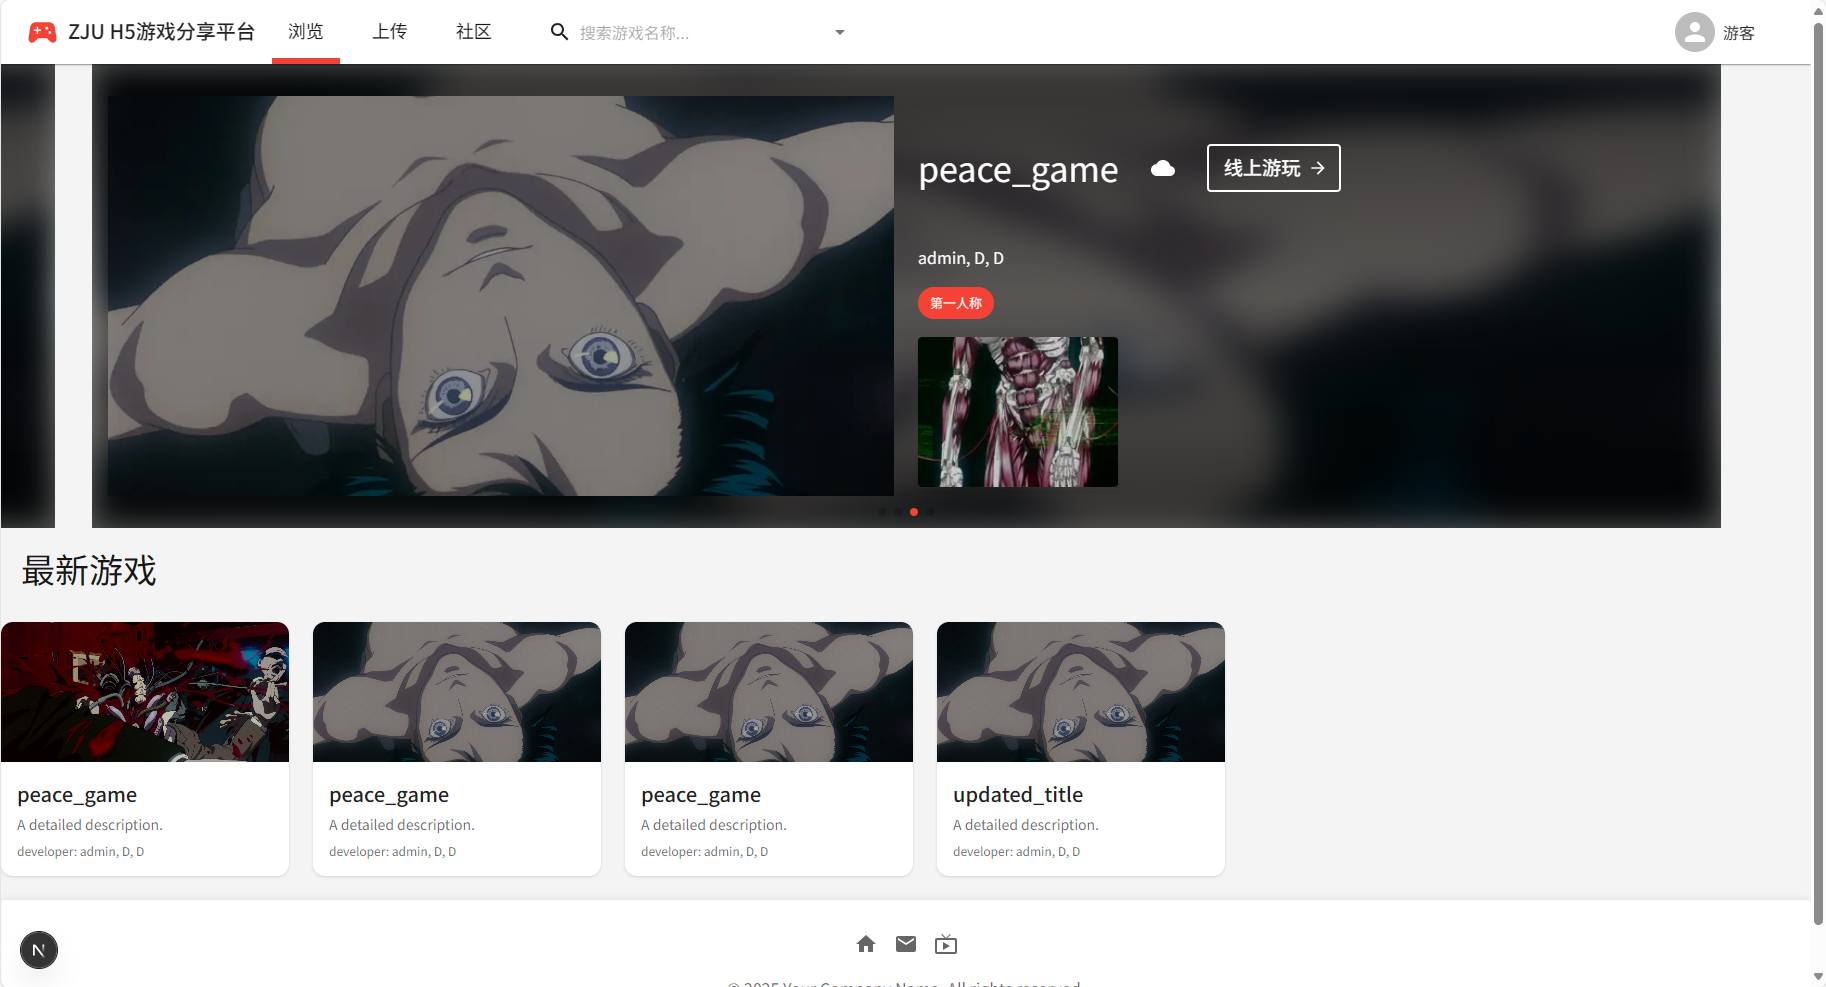
\includegraphics[width=0.8\textwidth]{mainwebpage.png}
  \caption{首页浏览页展示}
\end{figure}

用户可以通过点击其中任意的游戏封面,进入游戏详情页,如果用户上传的是 html 类型的游戏,即可在线游玩:

 \begin{figure}[H]
  \centering 
  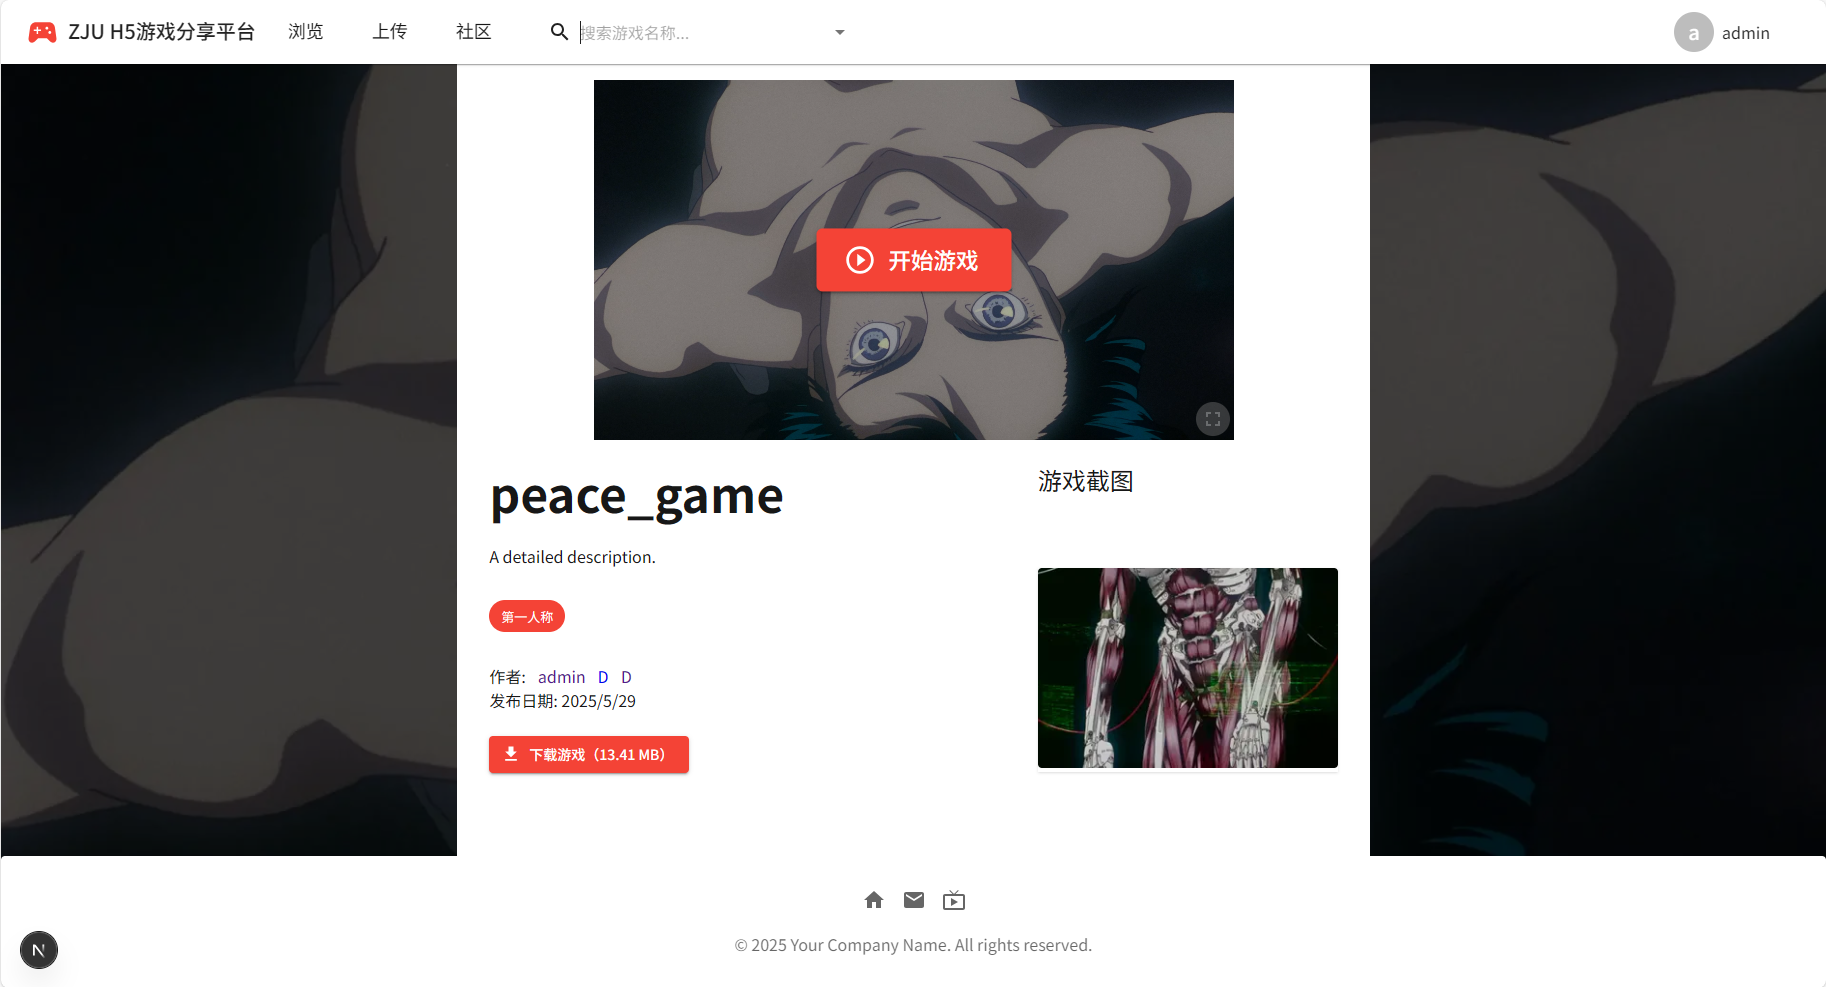
\includegraphics[width=0.8\textwidth]{homepage.png}
  \caption{游戏详情页展示}
\end{figure}

\subsubsection{登录界面}
登录界面是用户登录平台的入口,支持普通用户和管理员登录。用户可以输入用户名和密码进行身份验证。
\begin{figure}[H]
  \centering 
  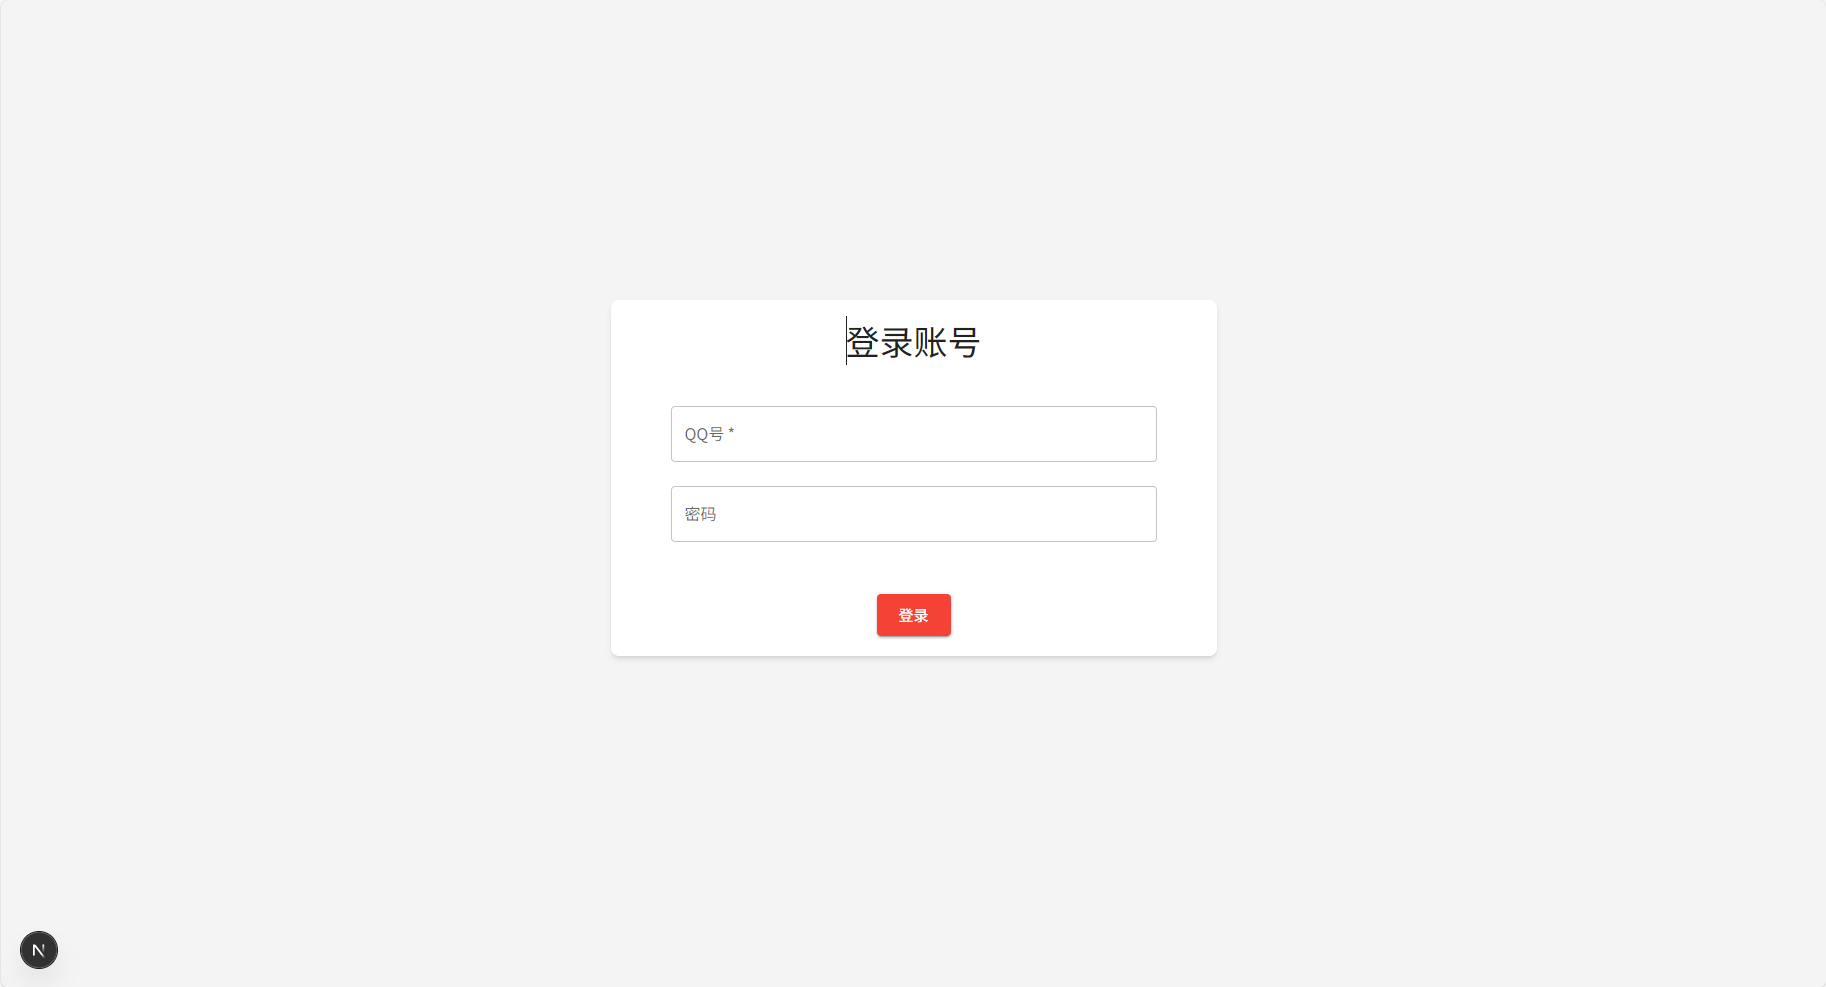
\includegraphics[width=0.8\textwidth]{login.png}
  \caption{登录界面}
\end{figure}
\subsubsection{用户界面}
用户界面展示了用户的个人信息、已上传的游戏列表等。用户可以在此界面进行个人信息修改和游戏管理。
\begin{figure}[H]
  \centering 
  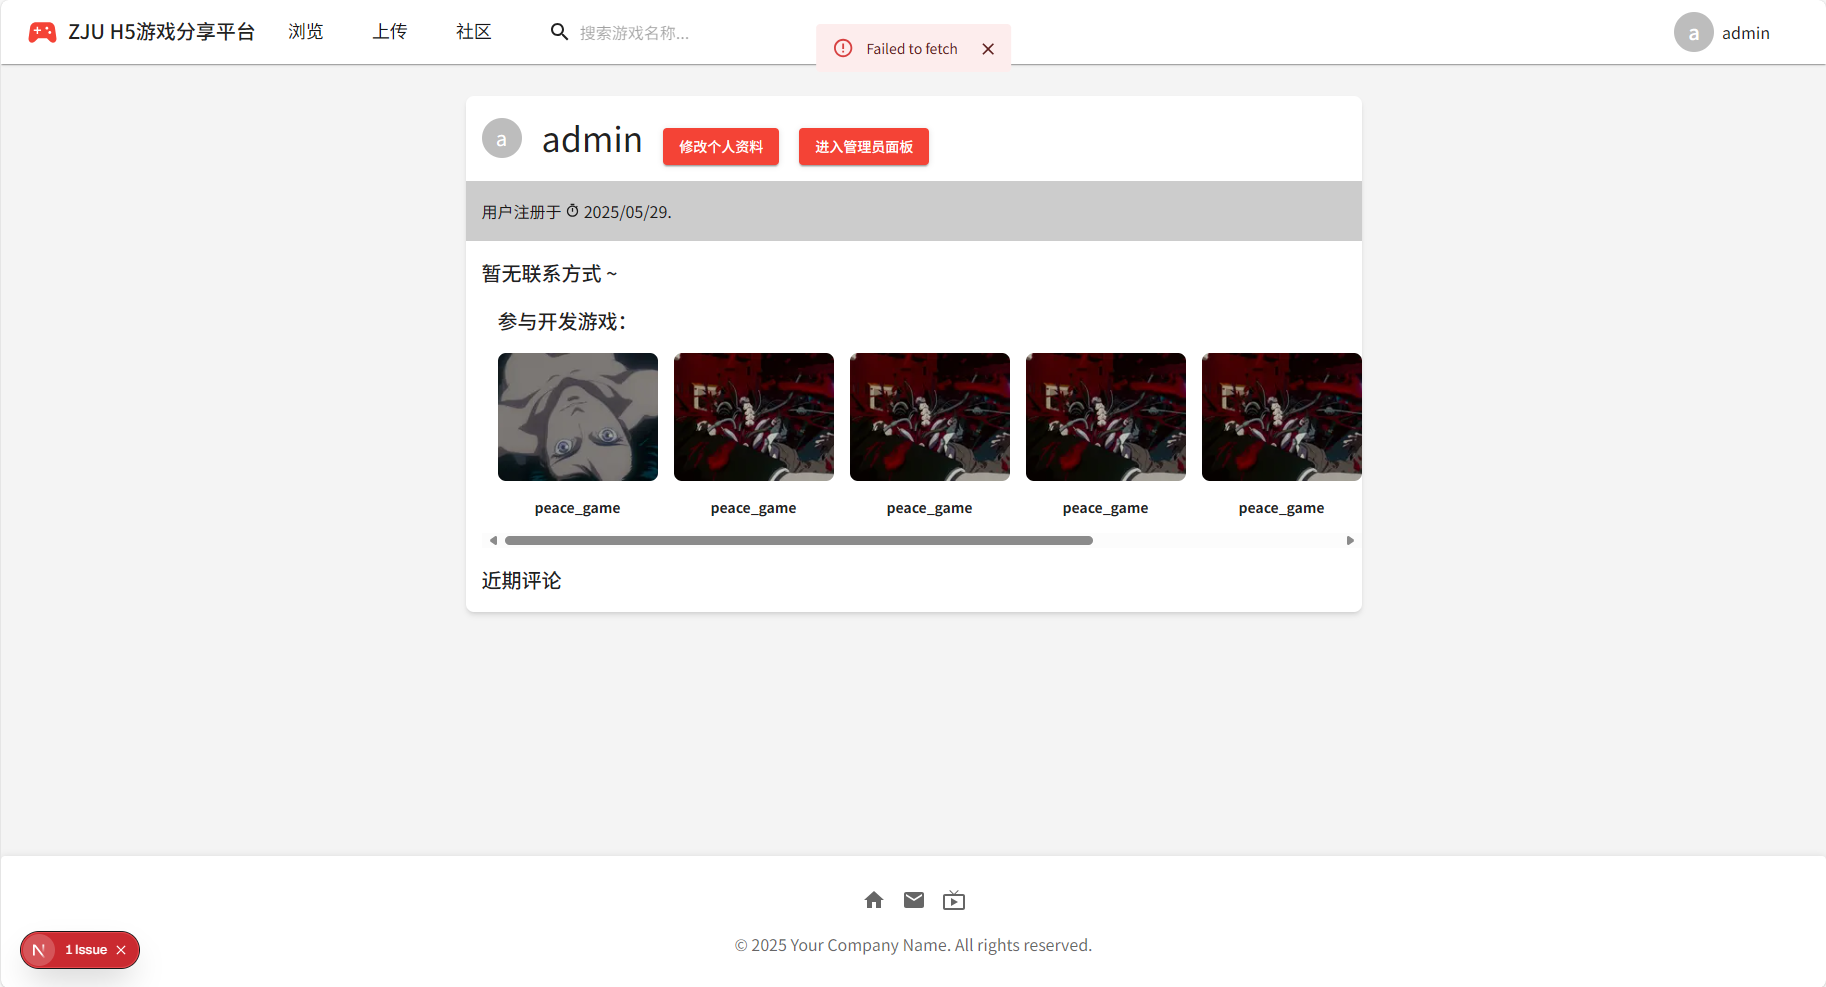
\includegraphics[width=0.8\textwidth]{userpage.png}
  \caption{用户界面}
\end{figure}
\subsubsection{用户信息更新界面}
 用户信息更新界面是普通用户修改个人信息的地方。用户可以在此界面进行个人信息修改。
\begin{figure}[H]
  \centering 
  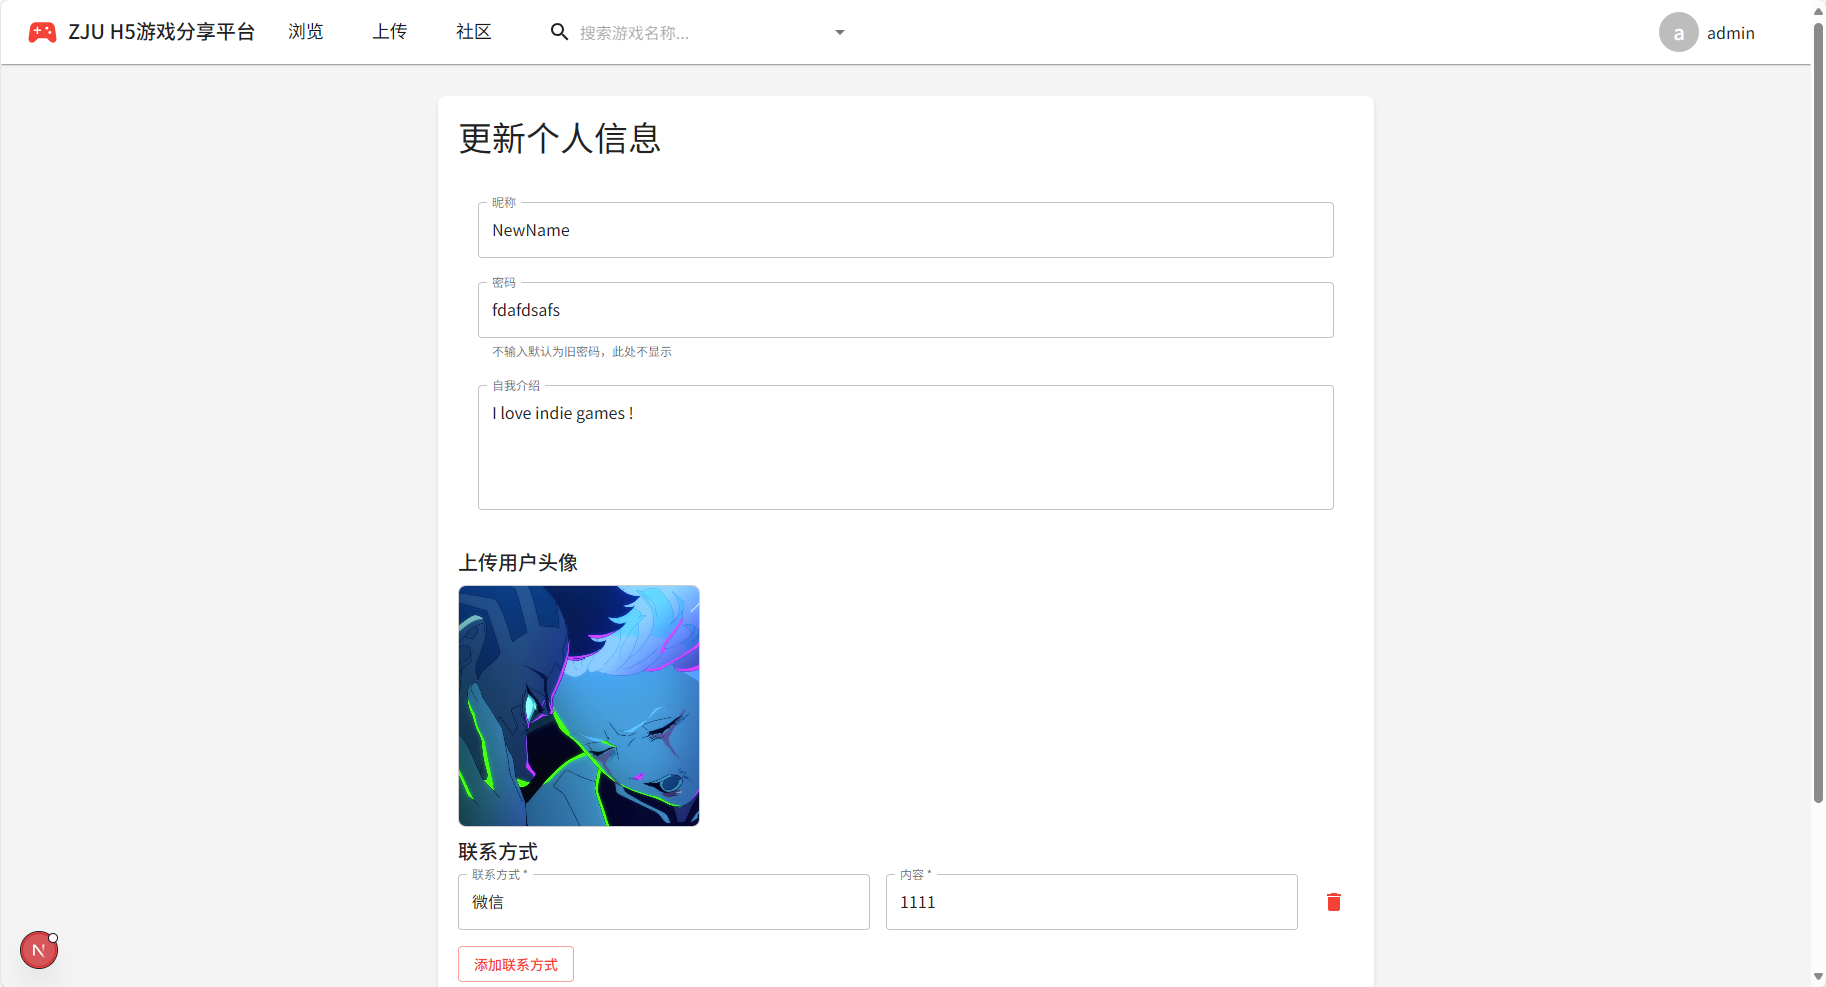
\includegraphics[width=0.8\textwidth]{userdataupdate.png}
  \caption{用户信息更新界面}
\end{figure}
\subsubsection{游戏上传界面}
游戏上传界面是普通用户和管理员上传新游戏或更新现有游戏信息的地方。用户可以填写游戏标题、描述、分类标签等信息,,并上传游戏文件和截图。
\begin{figure}[H]
   \centering
    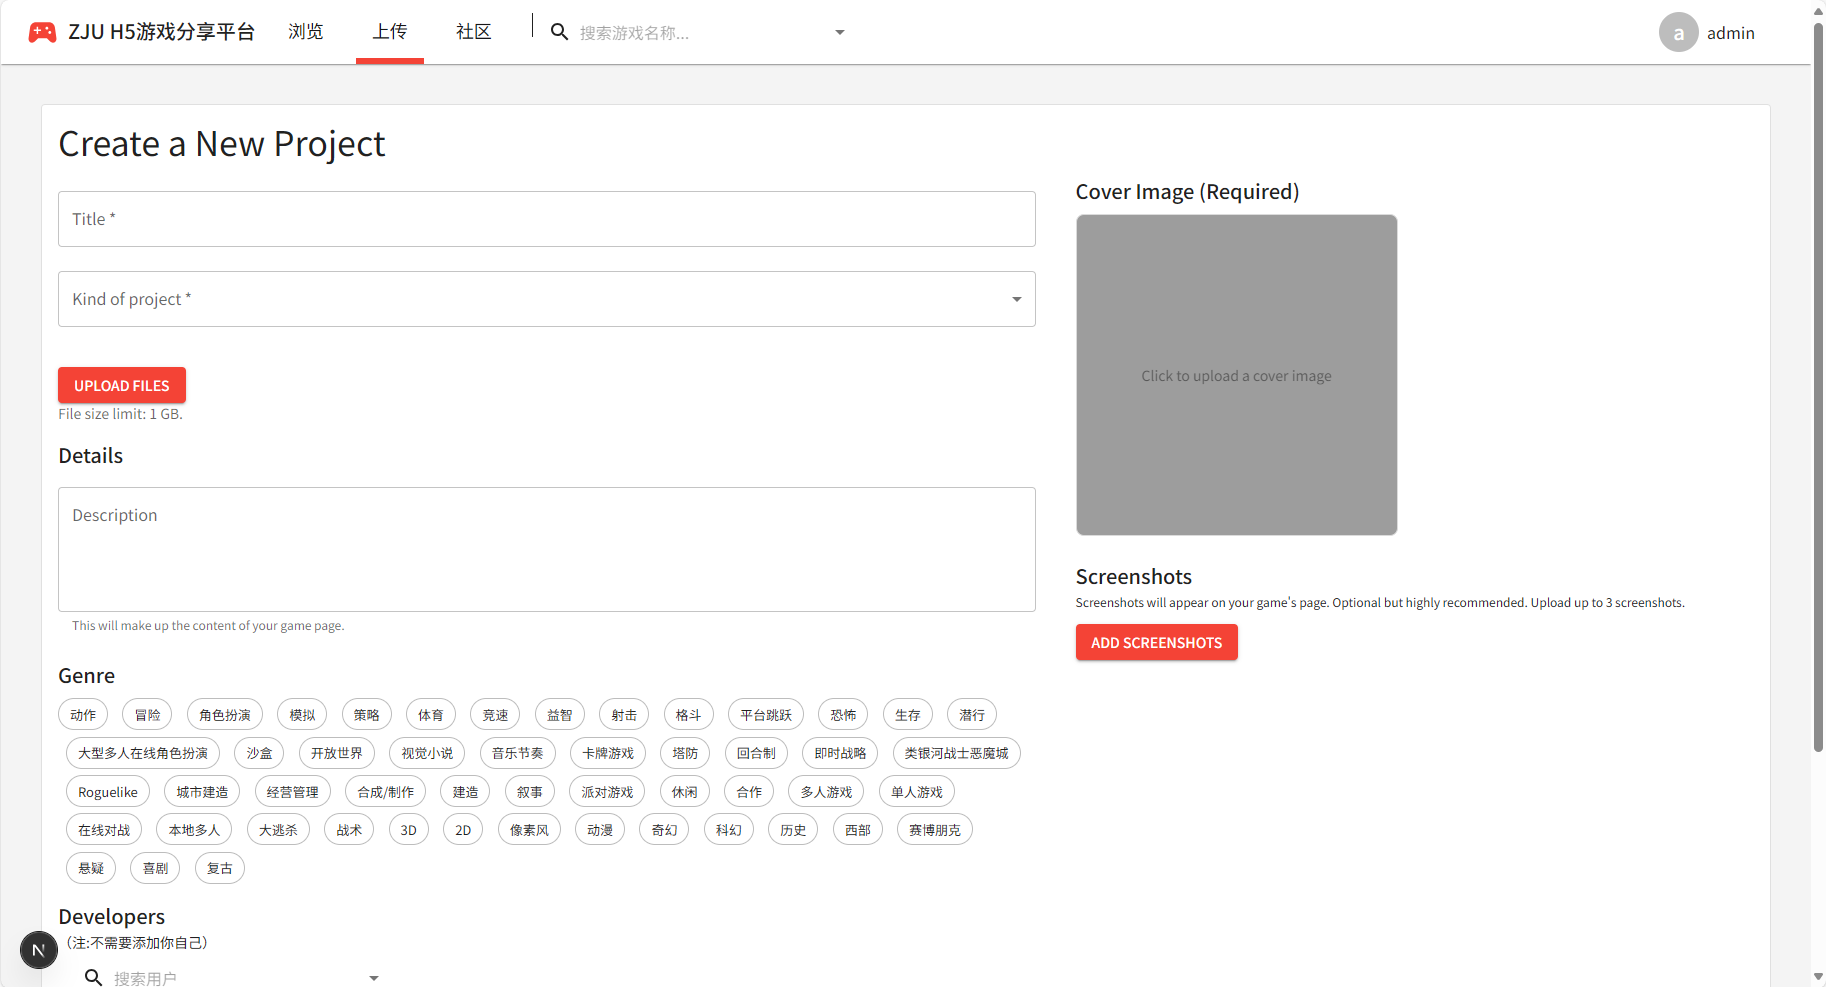
\includegraphics[width=0.8\textwidth]{updategame.png}
    \caption{游戏上传界面}
\end{figure}
\subsubsection{管理员界面}
 管理员界面是管理员管理游戏审核、游戏下架、用户的地方。管理员可以在此界面进行游戏管理、用户管理。
\begin{figure}[H]
  \centering 
  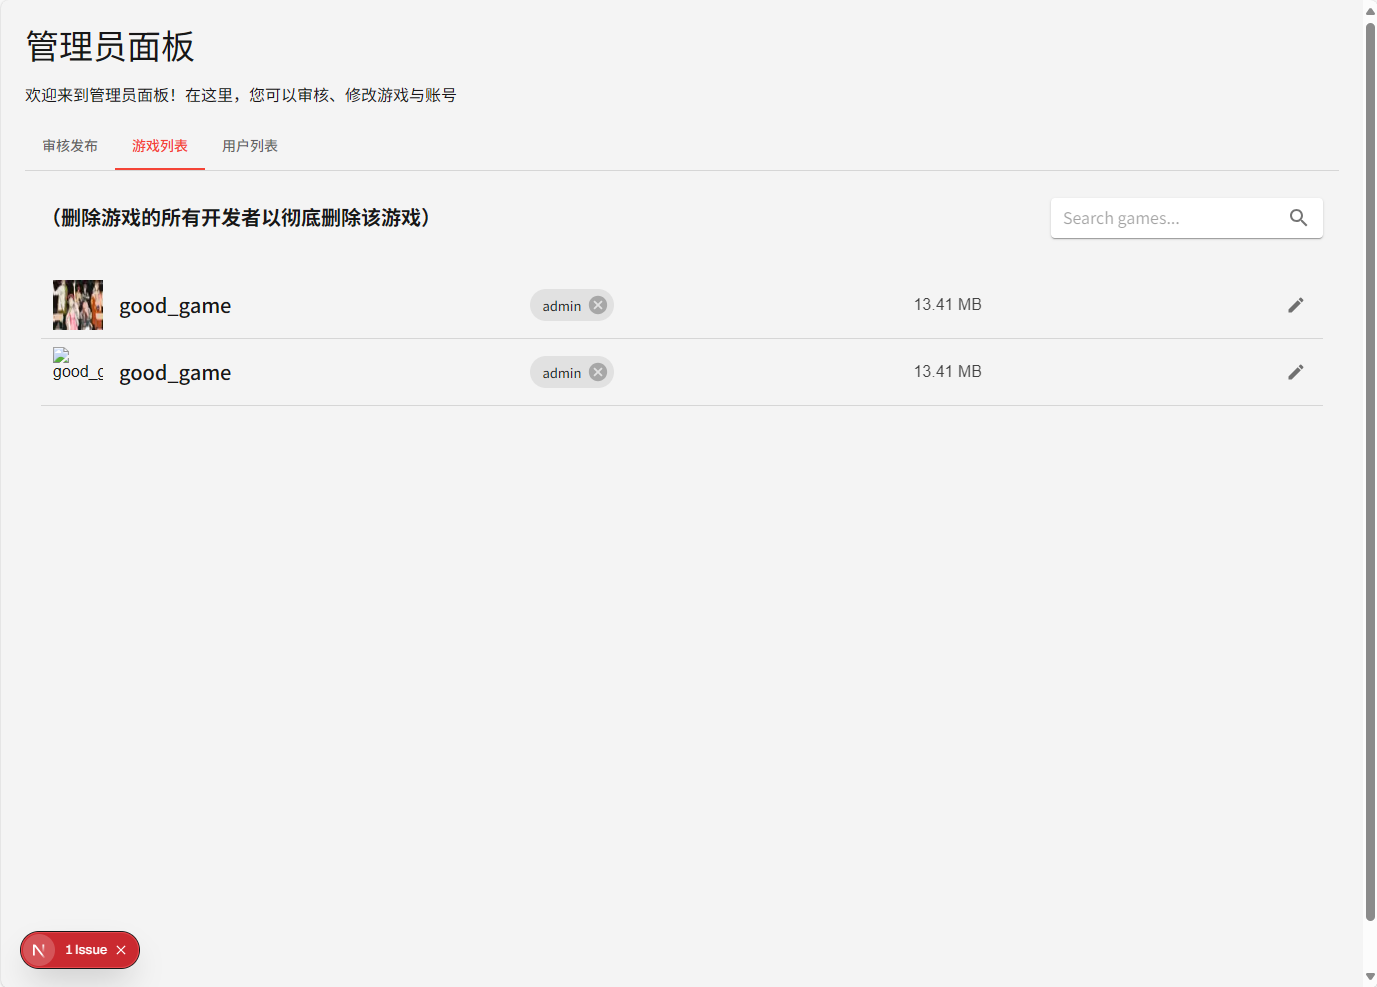
\includegraphics[width=0.8\textwidth]{managergame.png}
  \caption{游戏管理界面}
\end{figure}
\begin{figure}[H]
  \centering 
  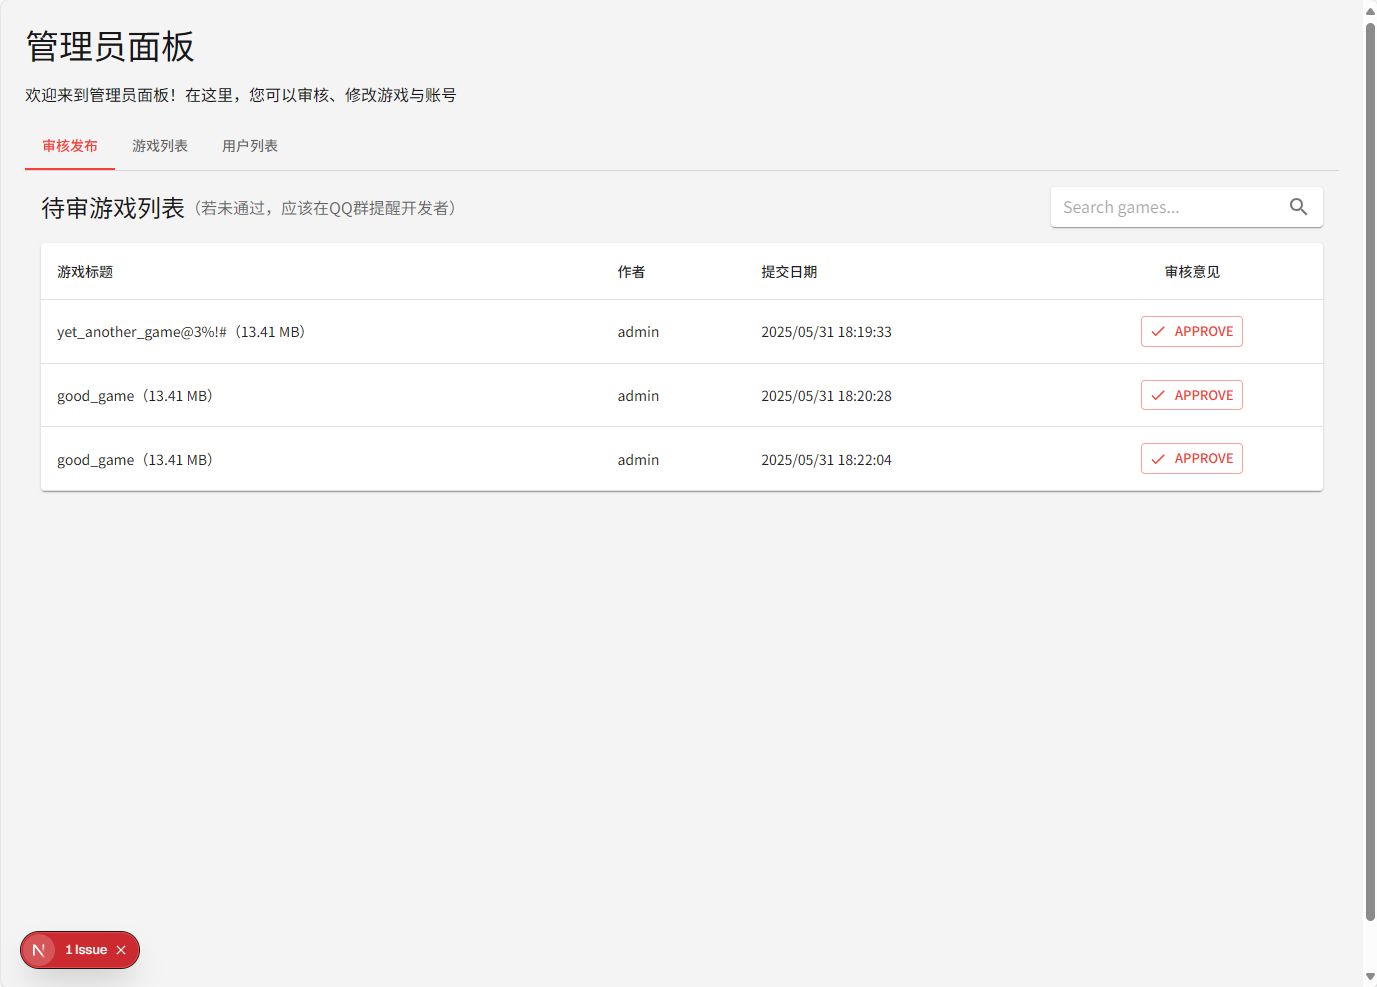
\includegraphics[width=0.8\textwidth]{managerunadited.png}
  \caption{未审核游戏管理界面}
\end{figure}
\begin{figure}[H]
  \centering 
  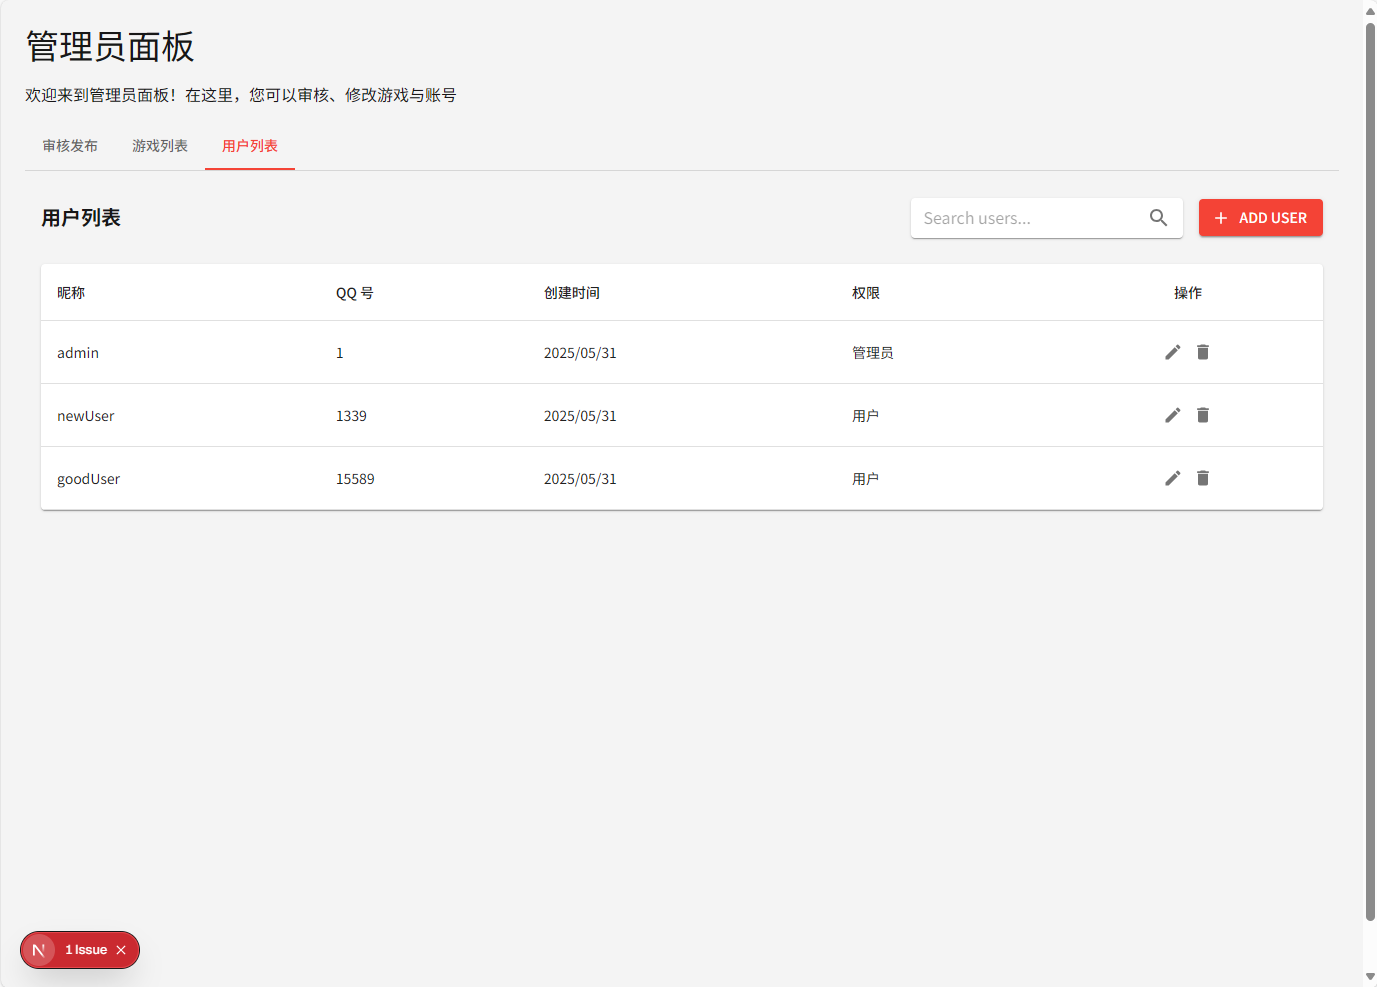
\includegraphics[width=0.8\textwidth]{manageruser.png}
  \caption{用户管理界面}
\end{figure}
\section{设计模式}
\subsection{概述}
设计模式可以让你避免从零开始设计你的产品,甚至在花费时间和精力后却最终设
计出一个不如别人现有产品的东西。通过使用现有的设计模式,你可以为特定问题获得
经过验证的解决方案。随着每种模式的应用,解决方案被整合,要构建的应用程序也就
逐渐更接近完整的设计。使用得当的设计模式,一定会对软件设计有巨大帮助。

在《设计模式:可复用面向对象软件的基础》一书中,提到了23种设计模式,这是设计
模式领域里程碑的事件,导致了软件设计模式的突破。这 4 位作者在软件开发领域里
也以他们的“四人组”(Gang of Four,GoF)匿名著称,这23种设计模式统称为GoF设
计模式,书中把它们分为创建型、结构型与行为型三种模式大类。我们也对GoF 所著的
设计模式书籍《设计模式:可复用面向对象软件的基础》进行了学习,并将其中提到的
设计模式与当前项目结合起来,具体如下。

\subsection{创建型模式} % 1. 创建型模式
\subsubsection{抽象工厂(Abstract Factory)} 
抽象工厂提供一个创建一系列相关或相互依赖对象的接口,而无需指定它们具体的类。
通过集中决定实例化哪个工厂,它的优点是具有较高的拓展性,当添加新的具体工厂时,无需修改已有代码。
客户端也无需知晓具体实现,只需要调用抽象接口即可。

在网站的UI设计中,我们就可以采用抽象工厂方法,设置抽象工厂类,来进行有关类的实现。
对于UI中的各种元素,如网站整体背景、按钮、图片背景、图标等等,client只需调用UIfactory进行生产,
即可得到不同类型(如明亮或黑暗)的网站元素。这样一来代码更加清晰,同时也实现了各个物品的解耦。
\begin{figure}[H]
  \centering
  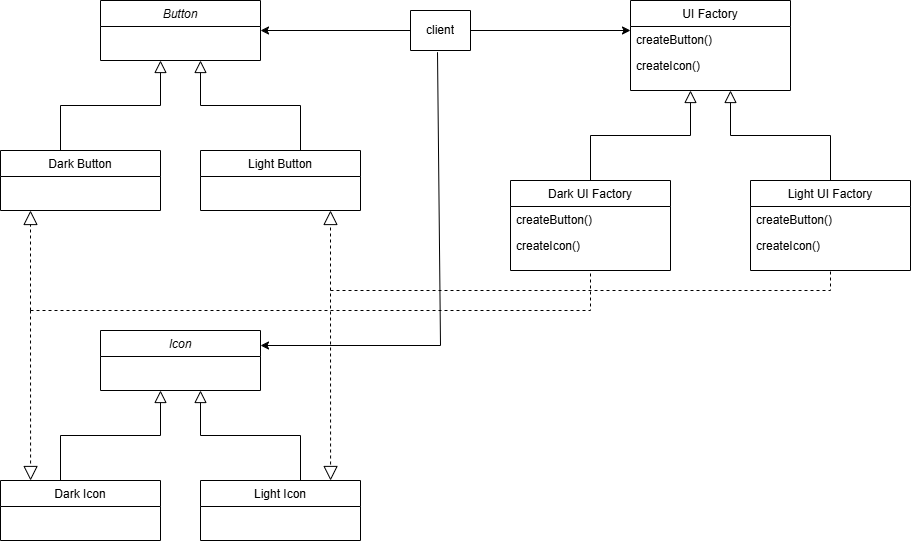
\includegraphics[width=\textwidth]{abs_factory.png}
  \caption{抽象工厂}
\end{figure}

\subsubsection{工厂方法(Factory Method)} 
工厂方法模式在父类中提供一个创建对象的方法,并允许子类决定实例化对象的类型。
这实际上是将类的实例化延迟至子类,使得创建对象的操作更加灵活而不必局限于类的直接创建。

对于浏览本网站的人,它们可能有着不同的身份(如不登录的游客、登录的用户等),因此我们可以单独实现一个类来对它们实现实例化,
而不是通过直接调用这些类自己的构造函数来实例化。如下图所示,client会调用工厂来生成/找到对应的visitor实例。
\begin{figure}[H]
  \centering
  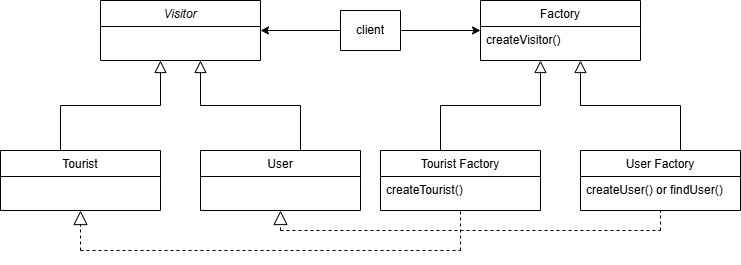
\includegraphics[width=0.8\textwidth]{factory_1.png}
  \caption{身份创建}
\end{figure}

由于在用户新上传游戏或者想要修改老游戏时,网页均会跳转到/upload页面,因此需要设计出一种既能处理新游戏,又能处理老游戏的方法。
事实上,这种复用现有对象的尝试也是工厂方法的一种应用。
通过复用,当处理老游戏时,它会在数据库种搜索对应的游戏id并进行数据展示和修改;而处理新游戏时则会新生成id并存储到数据库中。
\begin{figure}[H]
  \centering
  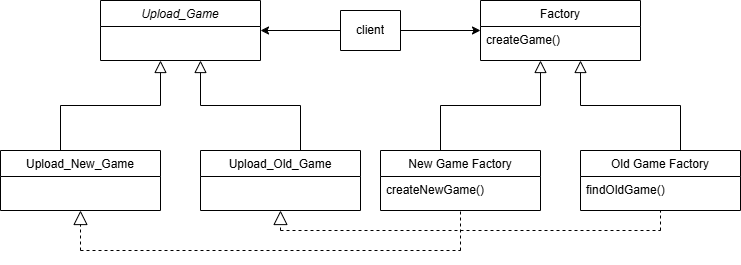
\includegraphics[width=0.8\textwidth]{factory_2.png}
  \caption{上传游戏的处理}
\end{figure}

\subsubsection{生成器(builder)} 
生成器这一设计模式帮助我们分步骤创建复杂对象,并允许使用相同的创建代码和步骤生成不同类型和形式的对象。

假设存在一个复杂对象,它包含许多子对象,因此其嵌套化的初始化导致了构造函数极其复杂。
为了解决这种问题,生成器模式建议将对象构造代码从产品类中抽取出来,并将其放在一个名为生成器的独立对象中。
接着它就会会将对象构造过程划分为一组步骤,并根据特定对象依次调用不同的步骤。

在我们的项目中,游戏对象就是一个明显的复杂对象,它具有较多属性如标题、描述、分类标签、开发者信息等,并且存在可选参数(截图等)。
因此,我们就可以用生成器分离构造过程与对象表示,支持链式调用。
\begin{figure}[H]
  \centering
  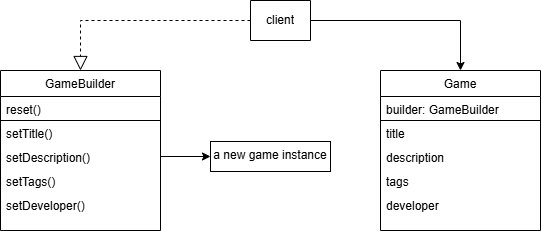
\includegraphics[width=0.8\textwidth]{builder.png}
  \caption{game对象生成}
\end{figure}

\subsubsection{原型(Prototype)} 
原型模式使你能够复制已有对象, 而又无需使代码依赖它们所属的类。
原型模式可以类比细胞的有丝分裂,也和C++代码中的拷贝构造函数有一定的相似性。

在我们的项目中,当我们需要整合某个游戏的不同版本时,我们可以用到原型模式,
并用拷贝构造函数进行实例化。在一个游客通过登录转换为新的正式用户时,
也可以使用原型模式复制一些已经记录的信息。
不过这些用法意义均不大,因此并没有实际应用。

\subsubsection{单件(Singleton)} 
单件模式让你能够保证一个类只有一个实例,并提供一个访问该实例的全局节点。
所有单例的实现都包含以下步骤:
将默认构造函数设为私有, 防止其他对象使用单例类的new运算符;
新建一个静态构建方法作为构造函数。该函数能够调用私有构造函数来创建对象,并将其保存在一个静态成员变量中。
此后所有对于该函数的调用都将返回这一缓存对象。

单件模式同时解决了两个问题,首先,它通过保证一个类只有一个实例,控制某些共享资源(例如数据库或文件)的访问权限。
具体而言,如果你创建了一个对象,同时过一会儿后你决定再创建一个新对象,此时你会获得之前已创建的对象,而不是一个新对象。
像报告中之前提到的各种工厂类其实就可以应用单件模式,因为工厂只需要一个即可。
\begin{figure}[H]
  \centering
  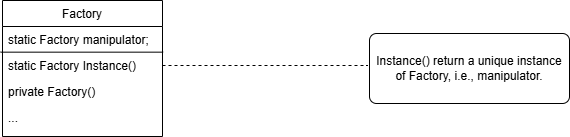
\includegraphics[width=0.8\textwidth]{singleton_1.png}
  \caption{工厂单件}
\end{figure}

其次,单件模式为该实例提供一个全局访问节点。类似于全局变量,它允许在程序的任何地方访问特定对象,并且能够保护该实例不被其他代码覆盖。
在我们的项目中,存储游戏数据以及管理文件的数据库就需要这样的全局访问性,所有的访问都会指向唯一的数据库。
\begin{figure}[H]
  \centering
  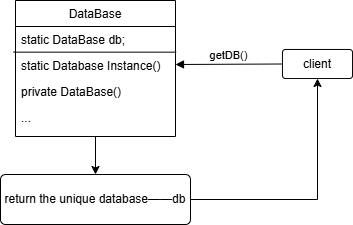
\includegraphics[width=0.8\textwidth]{singleton_2.png}
  \caption{数据库单件}
\end{figure}


\subsection{结构型模式} 
\subsubsection{适配器(Adaptor)} 
适配器模式,它允许接口不兼容的类能够一起工作。
适配器模式通过将一个类的接口转换成客户期望的另一个接口,解决了因接口不兼容而不能一起工作的类的问题。

适配器模式包含以下角色:
目标接口(Target): 客户期望的接口;
适配者(Adaptee): 需要被适配的现有接口;
适配器(Adapter): 将Adaptee接口转换为Target接口;

当代码有多人协作时,我们最初定义的类之间的接口调用可能不再得到实现,从
⽽导致接口相互不兼容,因此我们可以利用适配器模式来实现接口的兼容。
在我们的项目中,当我们对某些数据在不同部分没有严格契合,我们可以用到适配器模
式,并用在少修改代码的情况下引入新的适配器。
\begin{figure}[H]
  \centering
  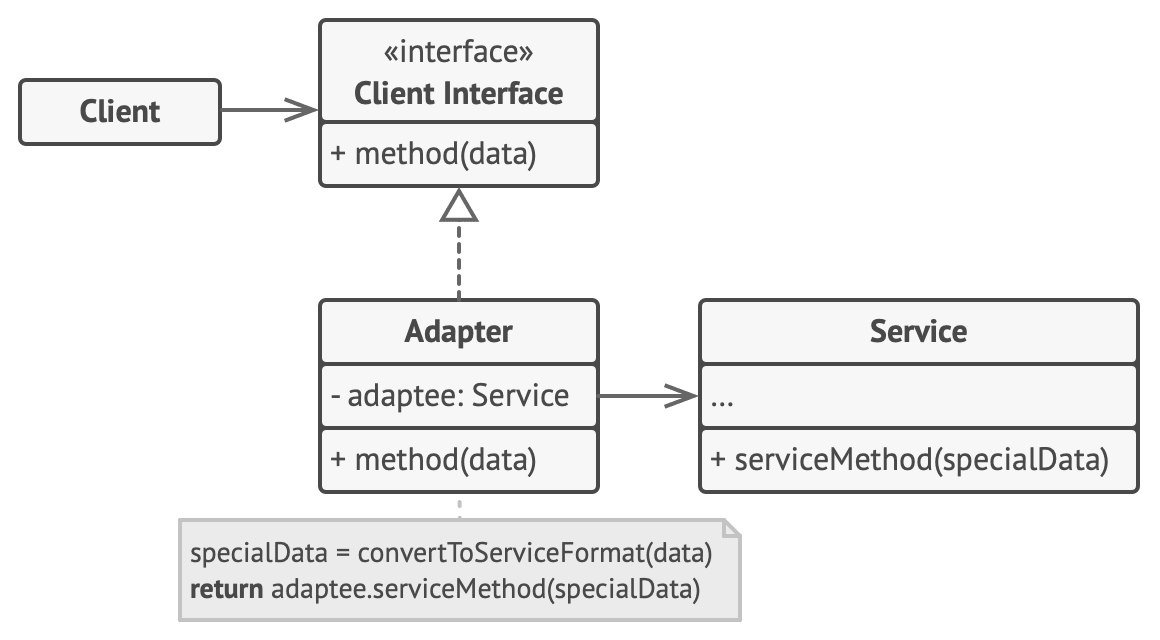
\includegraphics[width=0.7\textwidth]{shipei.png}
  \caption{适配器模式}
\end{figure}

\subsubsection{桥接(Bridge)} 
桥接模式,它将抽象部分与其实现部分分离,使它们可以独立变化。
该模式通过将继承关系改为组合关系来解决多层继承带来的类爆炸问题,
特别适用于一个类存在多个独立变化的维度时。具体来说, 
就是抽取其中一个维度并使之成为独立的类层次, 
这样就可以在初始类中引用这个新层次的对象, 从而使得一个类不必拥有所有的状态和行为。

桥接模式包含以下核心角色:
抽象部分(Abstraction):定义高层控制逻辑,依赖实现部分完成底层操作
扩展抽象(RefinedAbstraction):对抽象部分的扩展
实现部分接口(Implementor):定义实现类的接口
具体实现(ConcreteImplementor):实现Implementor接口的具体类

桥接模式具有两大特点:

解耦抽象与实现:允许抽象和实现独立扩展

提高可扩展性:新增抽象或实现类不影响现有代码

在我们的项目中,我们可以在多端存档同步系统的实现中使用桥接模式
在抽象层:存档数据模型;在实现层:可以有多种同步方式:云存储、本地缓存等
这样可以让我们在存档数据结构稳定情况下,灵活扩展新的同步渠道。
\begin{figure}[H]
  \centering
  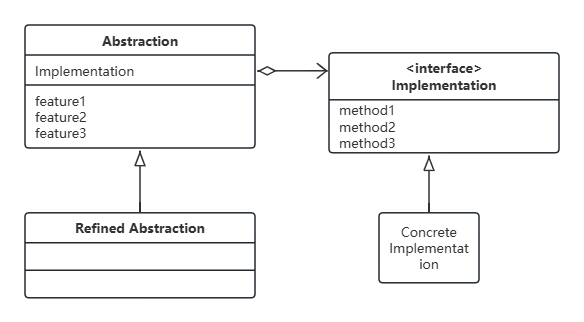
\includegraphics[width=0.7\textwidth]{qiaojie.png}
  \caption{桥接模式}
\end{figure}
\subsubsection{外观(Facade)} 
外观模式,它为复杂的子系统提供了一个简化的接口。
外观模式定义了一个高层接口,使得子系统更容易使用,同时仍然保持对子系统功能的完整访问能力。
其具有:简化接口,解耦,灵活的优点。

外观模式包含以下角色:
外观(Facade): 提供简化的接口,将客户端请求委派给适当的子系统对象;
子系统类(Subsystem classes): 实现子系统的功能,处理外观对象指派的工作;
客户端(Client): 通过外观接口与子系统交互

外观模式适用于以下情况:
需要为复杂的子系统提供一个简单的接口;
客户端与抽象的实现类之间存在很大的依赖性;
需要将子系统分层,使用外观模式定义每个层次的入口点;
我们可以使用外观模式实现
向多个数据分析平台(Google Analytics、腾讯云分析、自有分析系统)上报数据的需求。

\begin{figure}[H]
  \centering
  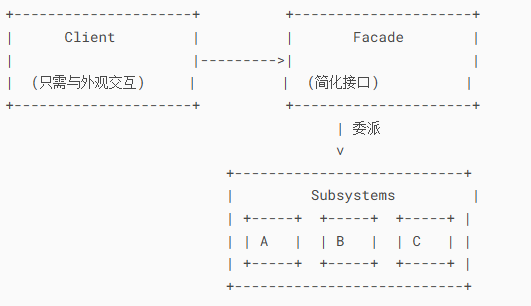
\includegraphics[width=0.7\textwidth]{waiguan.png}
  \caption{外观模式}
\end{figure}

\subsubsection{代理(Proxy)} 
代理模式,它为其他对象提供一种代理以控制对这个对象的访问。
代理对象在客户端和目标对象之间起到中介作用,可以在不改变原始类代码的情况下,
通过引入代理类来增加额外的功能。

代理模式包含以下主要角色:
抽象主题(Subject): 定义真实主题和代理主题的共同接口;
真实主题(Real Subject): 实现真实的业务逻辑;
代理(Proxy): 控制对真实主题的访问,并可以附加额外功能;

代理模式拥有以下优势:
控制访问: 控制客户端对真实对象的访问;
增强功能: 在不修改原始对象的情况下增加额外功能;
解耦: 将客户端与真实对象解耦;
灵活性: 可以根据需要创建不同类型的代理
\begin{figure}[H]
  \centering
  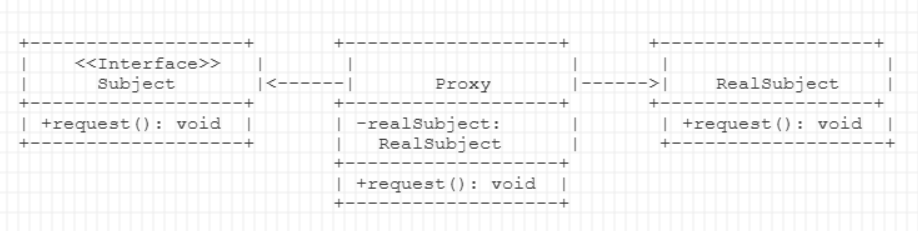
\includegraphics[width=1\textwidth]{daili1.png}
  \caption{代理模式}
\end{figure}

在我们的设计中: H5游戏需要加载大量资源(图片、音频、视频等),直接加载会影响用户体验。
我们可以进行以下的代理模式设计:使用虚拟代理实现资源的延迟加载和按需加载;
加载过程中显示占位图或加载动画;对加载失败资源进行智能替换或重试。
\begin{figure}[H]
  \centering
  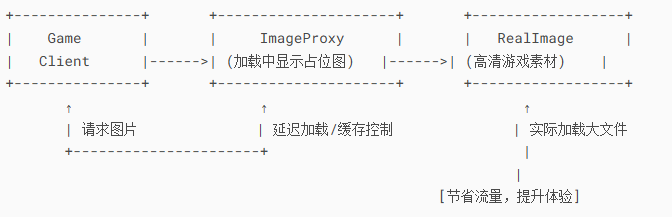
\includegraphics[width=1\textwidth]{daili2.png}
  \caption{应用示例}
\end{figure}
\subsection{行为模式}  
\subsubsection{迭代器(Iterator)} 
迭代器模式,它提供一种顺序访问聚合对象(如集合、列表、树等)中元素的方法,而无需暴露其底层表示。
其核心思想是将遍历逻辑与数据结构分离,使客户端可以统一处理不同类型的集合。
除实现自身算法外, 迭代器还封装了遍历操作的所有细节, 例如当前位置和末尾剩余元素的数量。 
因此, 多个迭代器可以在相互独立的情况下同时访问集合。

所有迭代器必须实现相同的接口。 这样一来, 只要有合适的迭代器, 客户端代码就能兼容任何类型的集合或遍历算法。 
如果你需要采用特殊方式来遍历集合, 只需创建一个新的迭代器类即可, 无需对集合或客户端进行修改。

在我们的设计中,通过使用迭代器模式,我们能较好地实现动态加载游戏资源(图片、音频等游戏数据),
避免一次性加载导致卡顿。同时可以相应实现按需加载资源,优化内存使用;支持优先级遍历(先加载关键资源)
\begin{figure}[H]
  \centering
  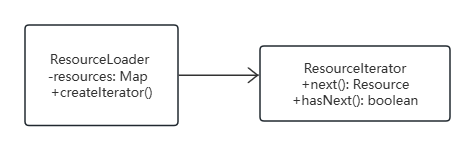
\includegraphics[width=1\textwidth]{diedai.png}
  \caption{迭代器模式示例}
\end{figure}
\subsubsection{备忘录(Memento)} 
备忘录模式,它允许在不破坏对象封装性的前提下,捕获并外部化对象的内部状态,以便后续可以恢复到这个状态。
其实现主要分为三个部分:Originator:需要保存状态的对象,提供创建/恢复备忘录的方法
Memento:存储Originator内部状态的对象(通常不可修改)
CareTaker:管理备忘录历史记录,但不直接操作备忘录内容

备忘录模式将创建状态快照 (Snapshot) 的工作委派给实际状态的拥有者原发器 (Originator) 对象。 
这样其他对象就不再需要从 “外部” 复制编辑器状态了, 编辑器类拥有其状态的完全访问权, 因此可以自行生成快照。
模式建议将对象状态的副本存储在一个名为备忘录 (Memento) 的特殊对象中。 
除了创建备忘录的对象外, 任何对象都不能访问备忘录的内容。 
其他对象必须使用受限接口与备忘录进行交互, 它们可以获取快照的元数据 (
创建时间和操作名称等), 但不能获取快照中原始对象的状态。

备忘录模式可以帮助我们实现玩家编辑的较为复杂的内容(如文字+截图)临时保存的功能,
更进一步的,可以实现玩家在不同设备上回复游戏进度,以及退回操作,即回档的功能。
\begin{figure}[H]
  \centering
  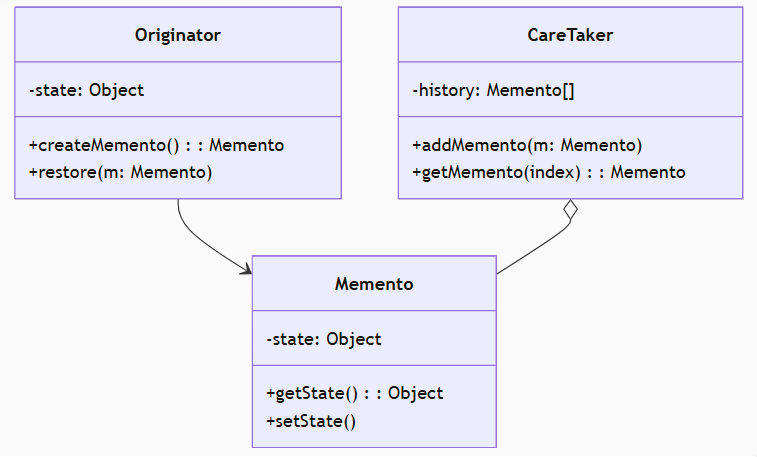
\includegraphics[width=1\textwidth]{beiwang.png}
  \caption{备忘录模式示例}
\end{figure}

\subsubsection{观察者(Observer)}
观察者模式它定义了一种一对多的依赖关系,
当一个对象(Subject)的状态发生改变时,所有依赖于它的对象(Observers)都会自动收到通知并更新。

拥有一些值得关注的状态的对象通常被称为目标, 由于它要将自身的状态改变通知给其他对象, 
我们也将其称为发布者 (publisher)。 所有希望关注发布者状态变化的其他对象被称为订阅者 (subscribers)
在实现中,所有订阅者都应该实现同样的接口, 发布者仅通过该接口与订阅者交互。 
接口中必须声明通知方法及其参数, 这样发布者在发出通知时还能传递一些上下文数据。
在我们的项⽬中,观察者模式可以应⽤在当游戏创作者通知收藏了自己游戏的用户(如游戏更新通知)
以及管理员像某些用户发送通知的功能上

\begin{figure}[H]
  \centering
  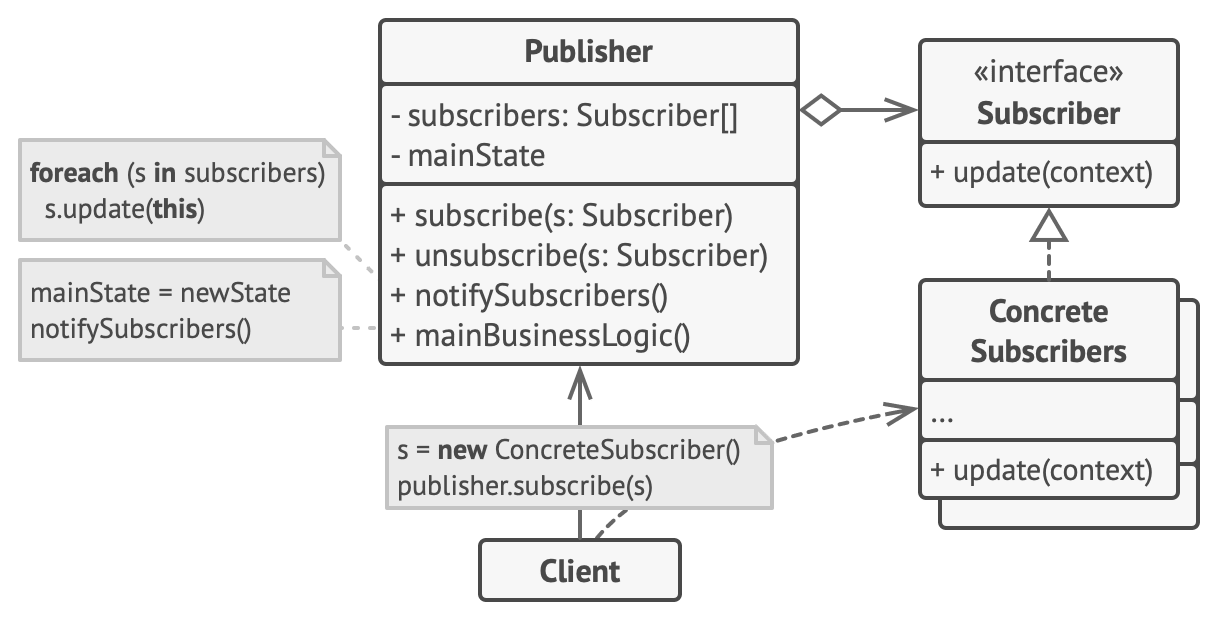
\includegraphics[width=1\textwidth]{guancha.png}
  \caption{观察者模式}
\end{figure}

\subsubsection{状态(State)} 
状态模式 能让你在一个对象的内部状态变化时改变其行为,使其看上去就像改变了自身所属的类一样。

状态模式与有限状态机 的概念紧密相关。
其主要思想是程序在任意时刻仅可处于几种有限的状态中。 在任何一个特定状态中, 程序的行为都不相同, 
且可瞬间从一个状态切换到另一个状态。不过,根据当前状态,
程序可能会切换到另外一种状态, 也可能会保持当前状态不变。 
这些数量有限且预先定义的状态切换规则被称为转移。
我认为其设计的核心功能有:
消除条件分支:用多态代替状态判断语句
状态封装:每个状态都是一个独立的类
动态切换:运行时自由切换状态对象

在我们的设计中,游戏玩家可能处于游客、已登录、封禁等不同状态,各状态下的功能权限不同
以及平台中的一些资源加载需处理初始化、加载中、就绪、失败等状态。
我们可以采用状态模式的设计来实现这些设计。

\begin{figure}[H]
  \centering
  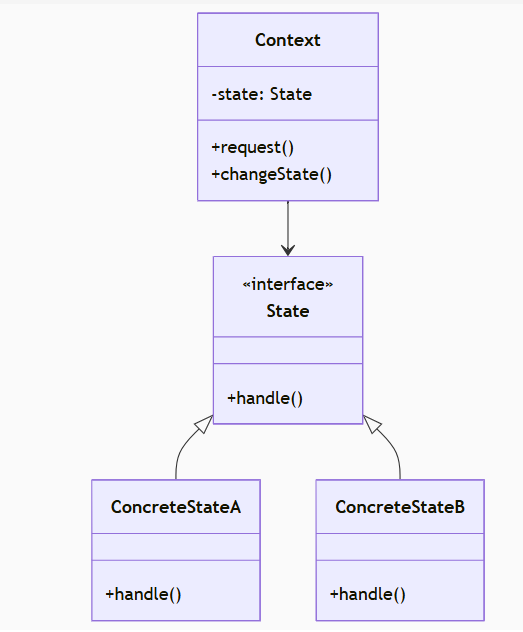
\includegraphics[width=1\textwidth]{zhuangtai.png}
  \caption{状态模式}
\end{figure}

\subsubsection{策略(Strategy)} 
策略模式中,它能让你定义一系列算法, 
并将每种算法分别放入独立的类中, 以使算法的对象能够相互替换,让算法的变化独立于使用它的客户端
同时可以让我们在运行时切换,动态选择最佳策略。

我们需要找出负责用许多不同方式完成特定任务的类, 然后将其中的算法抽取到一组被称为策略的独立类中。
名为上下文的原始类必须包含一个成员变量来存储对于每种策略的引用。 上下文并不执行任务, 
而是将工作委派给已连接的策略对象。

使用策略模式,我们可以对不同的用户设置符合他们的服务,如根据设备性能/屏幕尺寸自动调整UI布局
以提升不同设备用户的体验一致性,不同网络条件下的通信方案。

\begin{figure}[H]
  \centering
  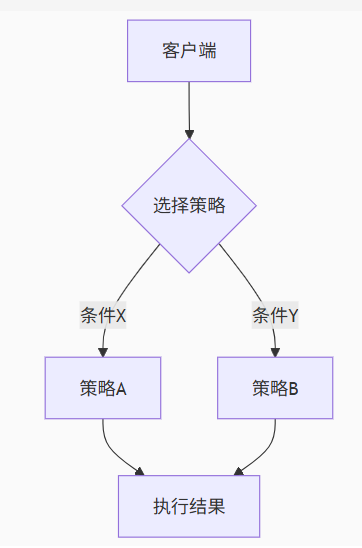
\includegraphics[width=0.8\textwidth]{celv.png}
  \caption{策略模式}
\end{figure}
\subsubsection{模板方法(Template Method)} 
模板方法模式它在一个方法中定义了一个算法的骨架,而将一些步骤延迟到子类中实现。
模板方法使得子类可以在不改变算法结构的情况下,重新定义算法中的某些步骤。
模板方法模式的设计可以实现标准化流程:固定算法执行顺序;
灵活扩展:子类可定制关键步骤;
避免重复:公共逻辑提升至父类

数据的上报需经过(收集→加密→压缩→传输),但加密/压缩方式因数据类型而异。
对此我们可以采用模板方法模式:

[数据上报模板]

├─ 1. 收集原始数据 (固定实现)

├─ 2. 执行数据加密 (抽象步骤)

├─ 3. 进行内容压缩 (抽象步骤)

└─ 4. 网络传输 (固定实现)

\begin{figure}[H]
  \centering
  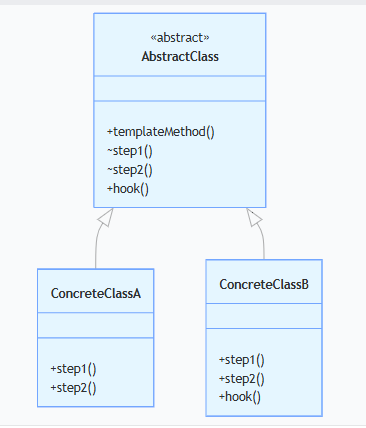
\includegraphics[width=0.8\textwidth]{moshi.png}
  \caption{模板方法模式}
\end{figure}
\section{测试}
\subsection{内容测试}
\begin{table}[H]
\centering
\renewcommand{\arraystretch}{1.5} 
\large
\begin{tabular}{|>{\centering\arraybackslash}m{10cm}|>{\centering\arraybackslash}m{3cm}|}
\hline
\textbf{测试内容} & \textbf{测试结果} \\
\hline
信息事实准确 & 通过 \\
\hline
信息简洁明了 & 通过 \\
\hline
内容布局易于用户理解 & 通过 \\
\hline
用户可以轻松找到内容对象中的信息 & 通过 \\
\hline
提供信息的正确引用或参考 & 通过 \\
\hline
呈现的信息不自相矛盾 & 通过 \\
\hline
内容不令人反感 & 通过 \\
\hline
内容没有误导性 & 通过 \\
\hline
内容的美学风格与界面的美学风格不冲突 & 通过 \\
\hline
\end{tabular}
\label{tab:test_results}
\end{table}

\subsection{数据库测试}
\begin{table}[H]
\centering
\Large
\caption{\Large postgresql数据库测试}
\renewcommand{\arraystretch}{1.5} 
\begin{tabular}{|>{\centering\arraybackslash}p{4cm}|>{\centering\arraybackslash}p{2cm}|>{\centering\arraybackslash}p{2cm}|>{\raggedright\arraybackslash}p{2cm}|}
\hline
\textbf{数据表} & \textbf{增} & \textbf{删}& \textbf{查} \\
\hline
games & 正常 & 正常 & 正常 \\
\hline
game\_images & 正常 & 正常 & 正常 \\ 
\hline
users & 正常 & 正常 & 正常 \\ 
\hline
user\_games & 正常 & 正常 & 正常 \\ 
\hline
\end{tabular}
\end{table}

\begin{table}[H]
\centering
\Large
\caption{\Large minio数据库测试}
\renewcommand{\arraystretch}{1.5} 
\begin{tabular}{|>{\centering\arraybackslash}p{4cm}|>{\centering\arraybackslash}p{2cm}|>{\centering\arraybackslash}p{2cm}|>{\raggedright\arraybackslash}p{2cm}|}
\hline
\textbf{桶} & \textbf{增} & \textbf{删}& \textbf{取} \\
\hline
games & 正常 & 正常 & 正常 \\
\hline
images & 正常 & 正常 & 正常 \\ 
\hline
photo & 正常 & 正常 & 正常 \\ 
\hline
\end{tabular}
\end{table}

\subsection{后端接口测试}
\begin{table}[H]
\centering
\renewcommand{\arraystretch}{1.5} 
\large
\begin{tabular}{|>{\centering\arraybackslash}m{8cm}|>{\centering\arraybackslash}m{5cm}|>{\centering\arraybackslash}m{3cm}|}
\hline
\textbf{测试内容} & \textbf{接口} & \textbf{测试结果}\\
\hline
获取游戏 & get/game & 通过\\
\hline
获取标签 & get/tag & 通过\\
\hline
获取用户 & get/user & 通过\\
\hline
用户登录 & put/user & 通过\\
\hline
上传游戏 & post/game & 通过\\
\hline
游戏更新 & put/game & 通过\\
\hline
用户信息更新 & put/user & 通过\\
\hline
用户登出 & delete/me & 通过\\
\hline
获取用户自身id & get/me & 通过\\
\hline
获取指定用户未审核游戏列表 & get/user\_game & 通过\\
\hline
管理员删除游戏 & delete/admin/game & 通过\\
\hline
管理员审核通过一个游戏 & put/admin/game & 通过\\
\hline
管理员删除用户 & delete/admin/user & 通过\\
\hline
管理员批量创建用户 & put/admin/user & 通过\\
\hline
管理员换绑 QQ 号 & put/admin/bind & 通过\\
\hline
\end{tabular}
\end{table}

\subsection{APIfox测试}
\begin{figure}[H]
  \centering
  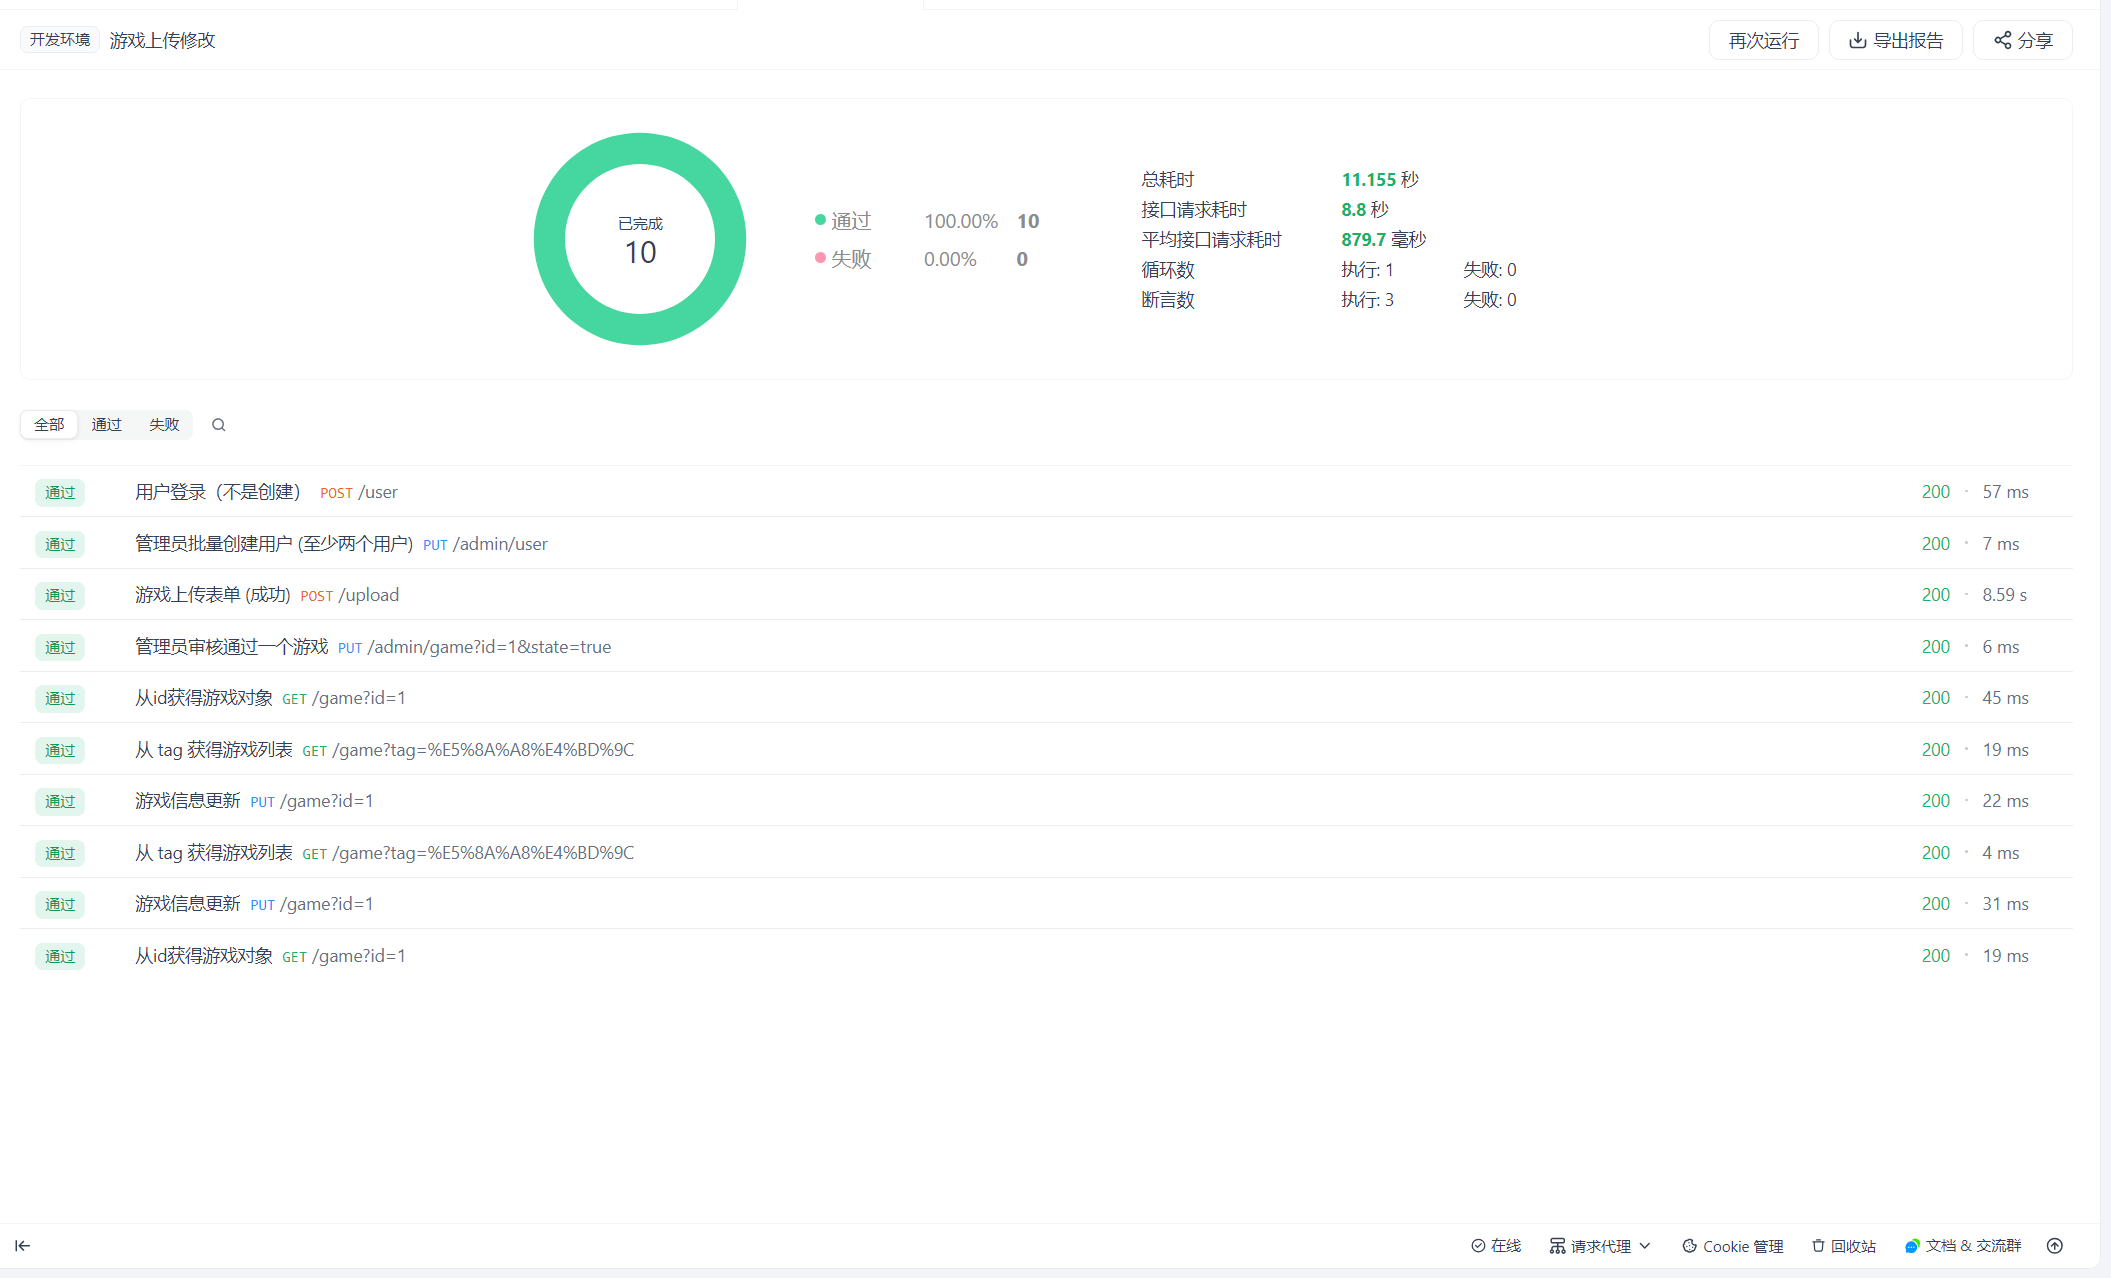
\includegraphics[width=\textwidth]{testresult1.png}
  \caption{游戏上传修改}
\end{figure}

\begin{figure}[H]
  \centering
  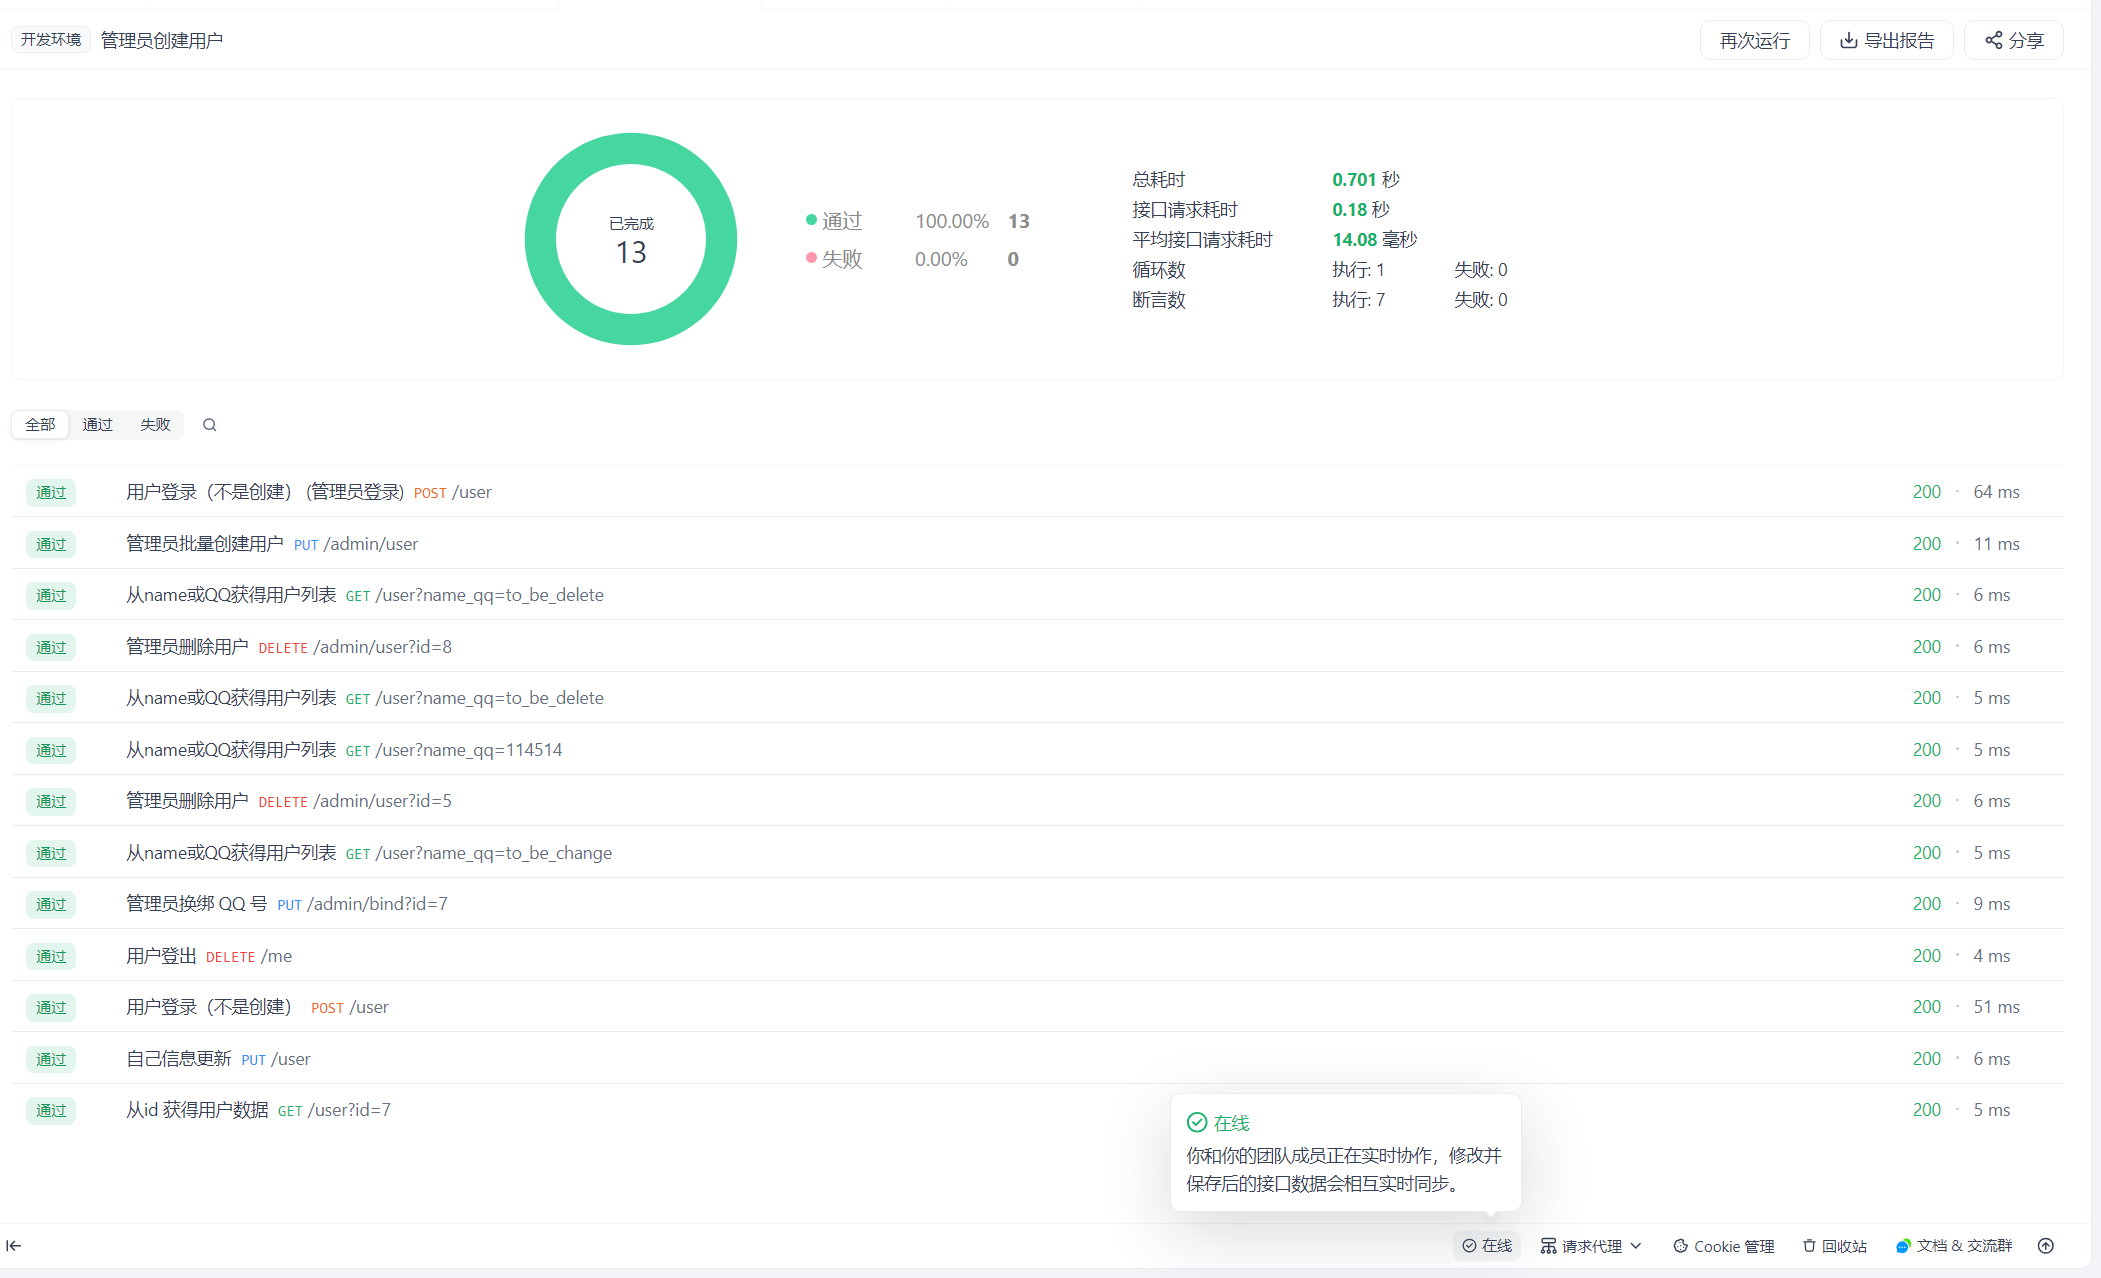
\includegraphics[width=\textwidth]{testresult2.png}
  \caption{管理员创建用户}
\end{figure}

\begin{figure}[H]
  \centering
  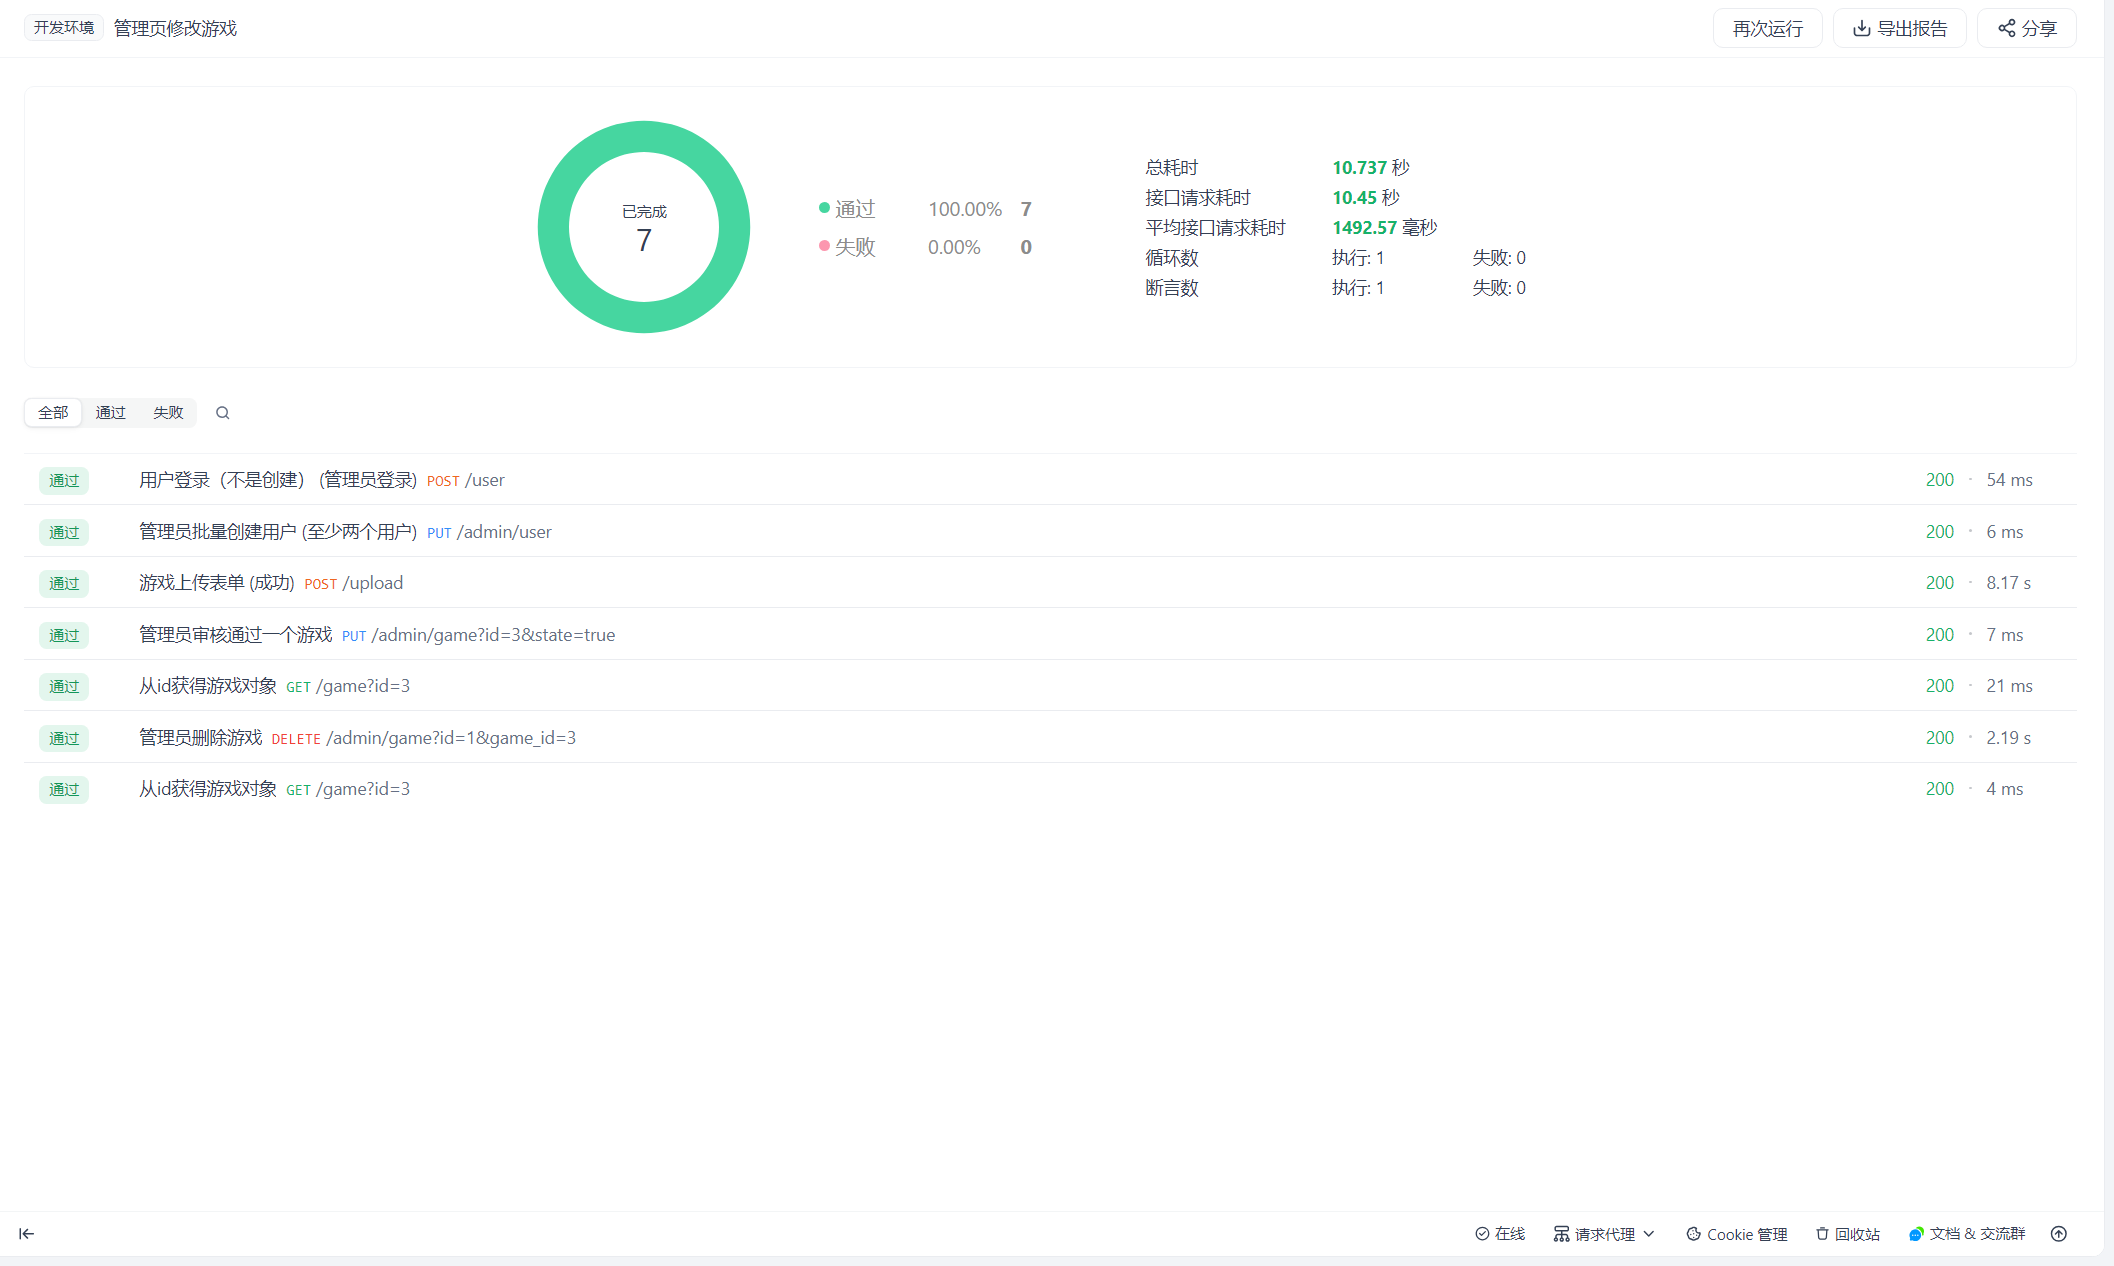
\includegraphics[width=\textwidth]{testresult3.png}
  \caption{管理员修改游戏}
\end{figure}

\subsection{边界测试}
\begin{table}[H]
\centering
\large
\renewcommand{\arraystretch}{1.5} 
\begin{tabular}{|>{\centering\arraybackslash}p{12cm}|>{\centering\arraybackslash}p{3cm}|>{\centering\arraybackslash}p{5cm}|>{\raggedright\arraybackslash}p{4cm}|}
\hline
\textbf{测试内容} & \textbf{测试结果} \\
\hline
 上传数据不合规的游戏上传表单 & 通过 \\
\hline
 游客请求无权限操作 & 通过 \\
\hline
 查找不存在游戏/用户 & 通过 \\
\hline
 登录时缺信息/信息错误 & 通过 \\
\hline
 管理员删改游戏输入不合规游戏id & 通过 \\
\hline
 管理员审核游戏输入错误游戏id & 通过 \\
\hline
\end{tabular}
\end{table}

\subsection{性能测试}
本地部署项目,我们对项目在一定负载情况下的表现进行测试。这里采用了ApiFox进行压力测试.
在并发20的情况下持续10分钟,我们的项目表现如下:
\begin{figure}[htbp]
  \centering 
  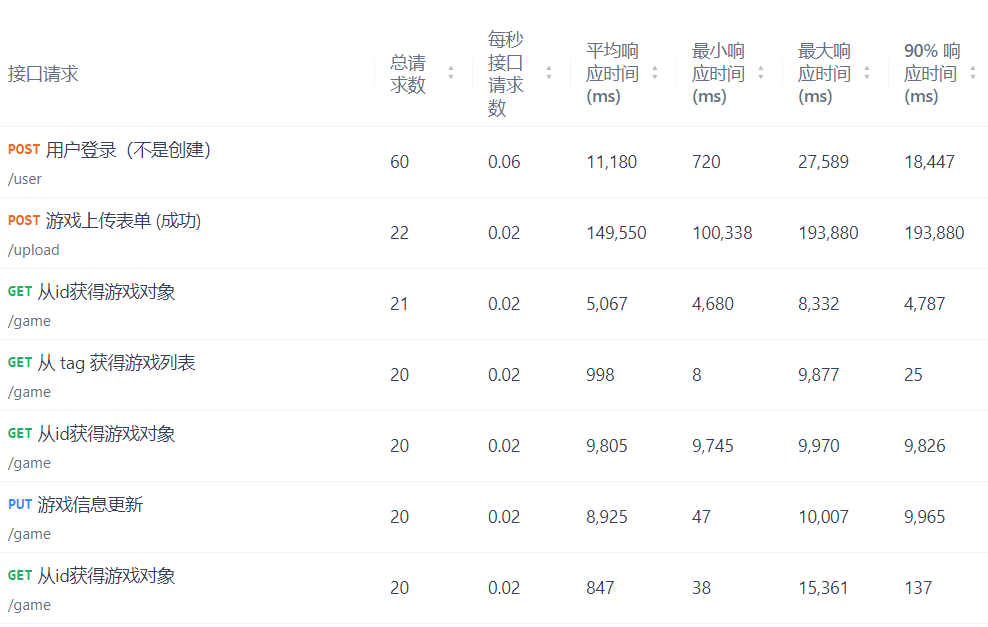
\includegraphics[width=1\textwidth]{test1.png}
\end{figure}

在低并发的情况下,未发现功能性错误,但在处理游戏大文件时存在的处理慢的问题会导致并发下的响应时间
为正常情况的两倍左右。当只有一名用户一直重复发送请求时,未发现功能性错误,响应时间正常。
并发用户达到100时出现错误,本项目目前并不支持高并发。

\subsection{总结分析}
通过此次测试,我们看到项目的一些优点,更看到了存在的一些问题。主要存在的问
题是项目对游戏大文件处理慢,不支持高并发;另外项目的功能也存在不
够完善的地方。我们会在接下来的开发过程中针对目前存在的问题进行改进。
\end{document}